\documentclass{article}
\usepackage[utf8]{inputenc}
\usepackage[left=1cm, right=1cm, top=2cm, bottom=2cm]{geometry}
\usepackage{graphicx}
\usepackage{caption}
\usepackage{subcaption}
\usepackage{amsmath}
\usepackage{booktabs} 
\usepackage{float}
\usepackage[colorlinks=true, urlcolor=blue, linkcolor=blue, citecolor=blue]{hyperref}
\usepackage{cleveref}

\title{Project 1}
\author{Masum Billah, Madhu Chencharapu, Gabriel Loos, Brendan McDonnell, Roshan Ravichandran}
\date{February 2026}

\begin{document}

\maketitle

\section{Introduction}

In this project, we will explore three different datasets using Neural Networks (2, 3, and 4 layers). The three datasets we will be using are:

\begin{itemize}
	\item \textbf{Auto MPG:} This dataset contains information about different cars. The goal is to predict the miles per gallon (MPG) given the other characteristics of the car. The dataset can be found at \url{https://archive.ics.uci.edu/dataset}.
	\item \textbf{California Housing Prices:} This dataset contains information about different housing locations. The goal is to predict the median house price of the area given the other characteristics. The dataset can be found at \url{https://www.kaggle.com/datasets/camnugent/california-housing-prices}.
	\item \textbf{Insurance Charges:} This dataset contains information about different primary beneficiaries of health insurance. The goal is to predict the primary beneficiaries insurance charges given their other characteristics. The dataset can be found at \url{https://www.kaggle.com/datasets/mirichoi0218/insurance}.
\end{itemize}

\section{Auto MPG}

\subsection{2 Layer Neural Network}

In Scalation, the best results were found when using the reLU as the activation function, a learning rate of $0.001$, and a batch size of $1$. Since the Auto MPG dataset is relatively small, picking a batch size of $1$ does not take much time, so is worth the better results, which are shown in \Cref{tab:Scalation - Auto MPG 2L NN}. In PyTorch, the best results were found when using the reLU as the activation function, a learning rate of $0.01$, and a batch size of $32$. The results are shown in \Cref{tab:PyTorch - Auto MPG 2L NN}. Plots for In-Sample and Out-of-Sample testing can be found in \Cref{fig:Auto MPG 2L Plots}.

\begin{table}[H]
\centering
\caption{Scalation - Auto MPG 2L NN}
\label{tab:Scalation - Auto MPG 2L NN}
\begin{tabular}{|c|c|c|} \hline 
Metric & In-Sample & 80-20 Split \\ \hline \hline 
rSq &0.727231 & 0.836932 \\ \hline 
rSqBar &0.722259 &      0.833959 \\ \hline 
sst &23819.0 &  4731.23 \\ \hline 
sse &6497.08 &  771.514 \\ \hline 
sde &3.39572 &  3.16498 \\ \hline 
mse0 &16.5742 & 9.89121 \\ \hline 
rmse &4.07114 & 3.14503 \\ \hline 
mae &3.31165 &  2.36625 \\ \hline 
smape &14.4265 &        10.7664 \\ \hline 
m &392.000 &    78.0000 \\ \hline 
dfr &7.00000 &  7.00000 \\ \hline 
df &384.000 &   384.000 \\ \hline 
fStat &146.255 &        281.549 \\ \hline 
aic &-1105.39 & -184.051 \\ \hline 
bic &-1073.62 & -165.198 \\ \hline 
\end{tabular}
\end{table}

\begin{table}[H]
\centering
\caption{PyTorch - Auto MPG 2L NN}
\label{tab:PyTorch - Auto MPG 2L NN}
\begin{tabular}{|c|c|c|}\hline
Metric & In-Sample & 80-20 Split \\ \hline \hline
rSq & 0.8232 & 0.8391 \\ \hline
rSqBar & 0.8199 & 0.8232 \\ \hline
sst & 23818.9935 & 4910.2699 \\ \hline
sse & 4211.9875 & 790.2830 \\ \hline
sde & 3.3119 & 3.3363 \\ \hline
mse0 & 10.7449 & 10.0036 \\ \hline
rmse & 3.2779 & 3.1628 \\ \hline
mae & 2.4941 & 2.4081 \\ \hline
smape & 11.4175 & 11.1501 \\ \hline
m & 392.0000 & 79.0000 \\ \hline
dfr & 8.0000 & 8.0000 \\ \hline
df & 384.0000 & 71.0000 \\ \hline
fStat & 223.4423 & 46.2681 \\ \hline
aic & 946.7758 & 197.9325 \\ \hline
bic & 978.5459 & 216.8881 \\ \hline
\end{tabular}
\end{table}

\begin{figure}[H]
     \centering
     \captionsetup{justification=centering}
     % First Row
     \begin{subfigure}[b]{0.4\textwidth}
         \centering
         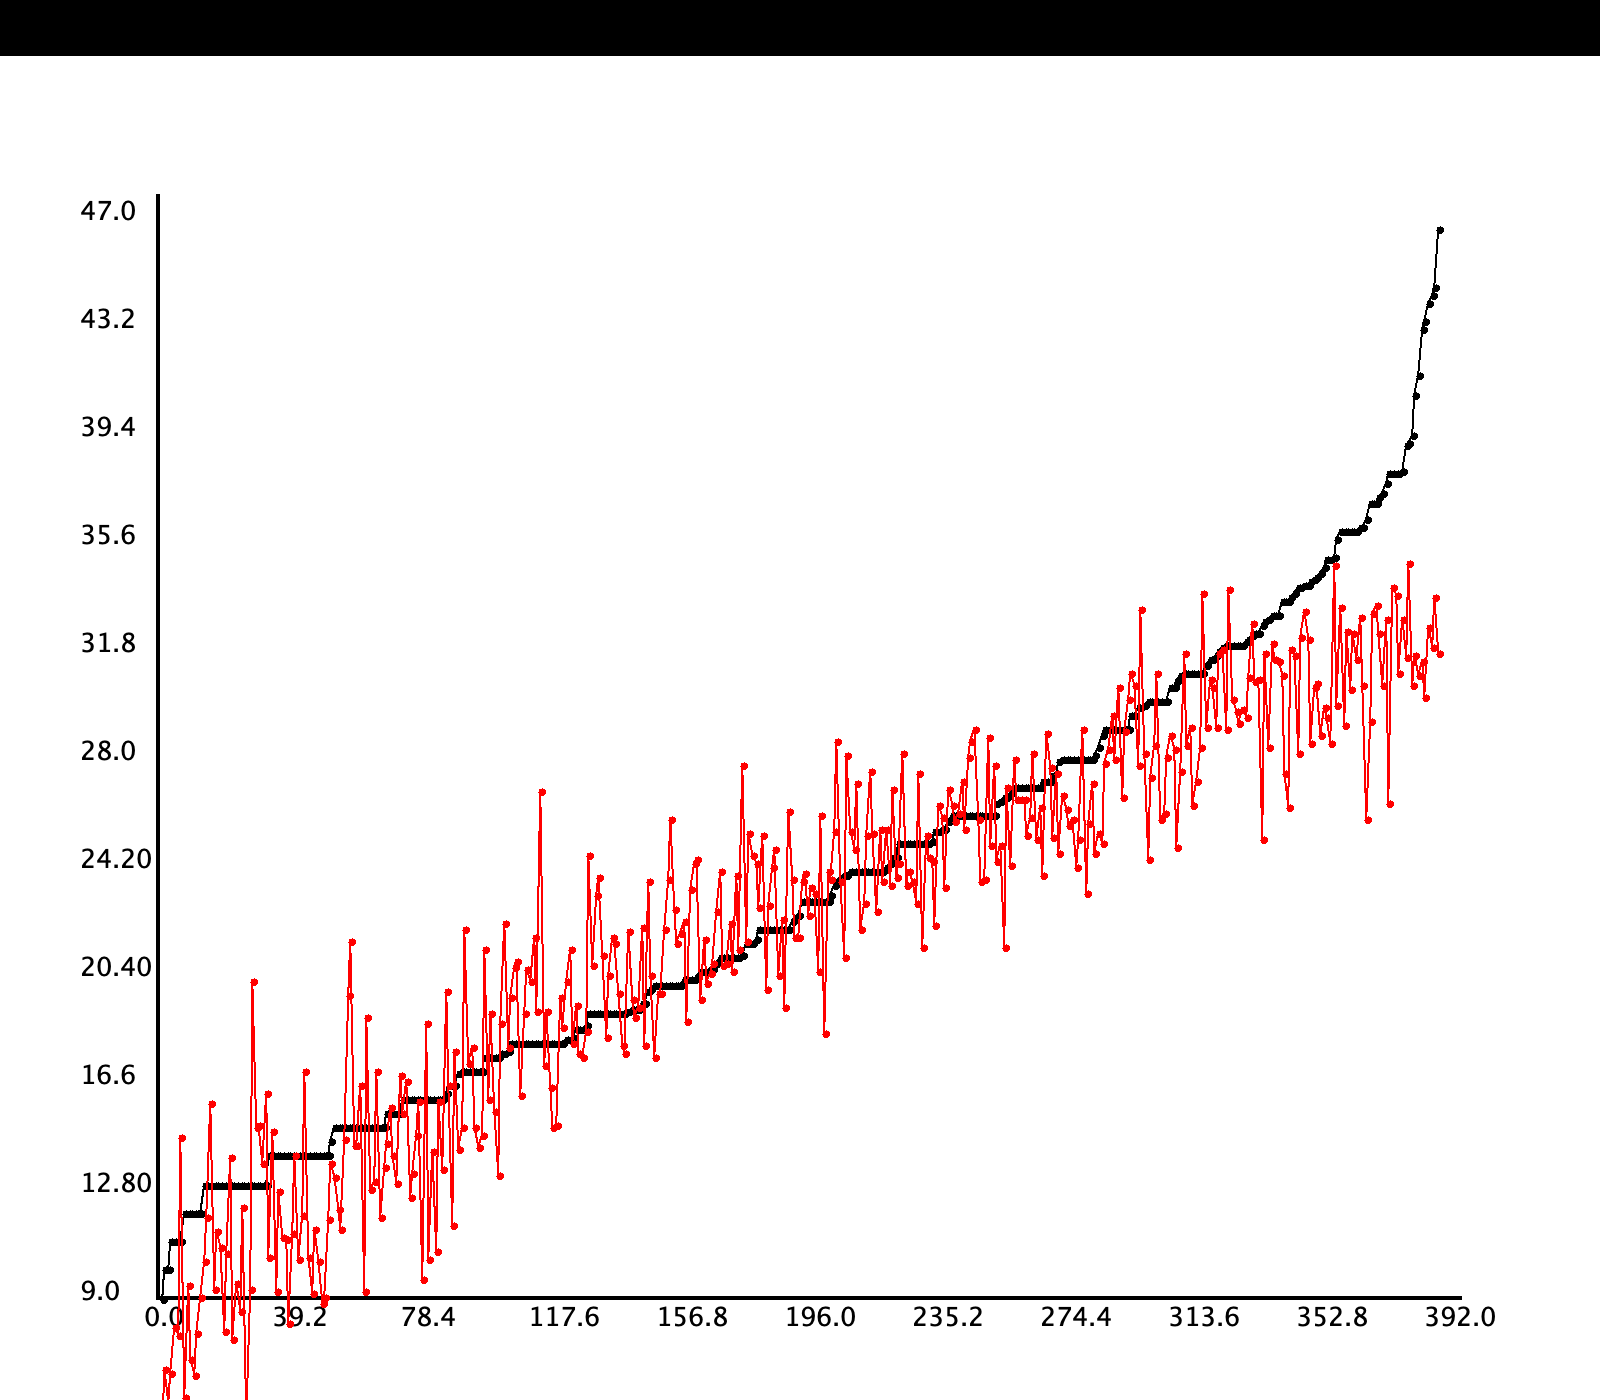
\includegraphics[width=\textwidth]{../Auto_MPG_P2/Scalation_2L_In_Sample.png}
     \end{subfigure}
     \hfill
     \begin{subfigure}[b]{0.4\textwidth}
         \centering
         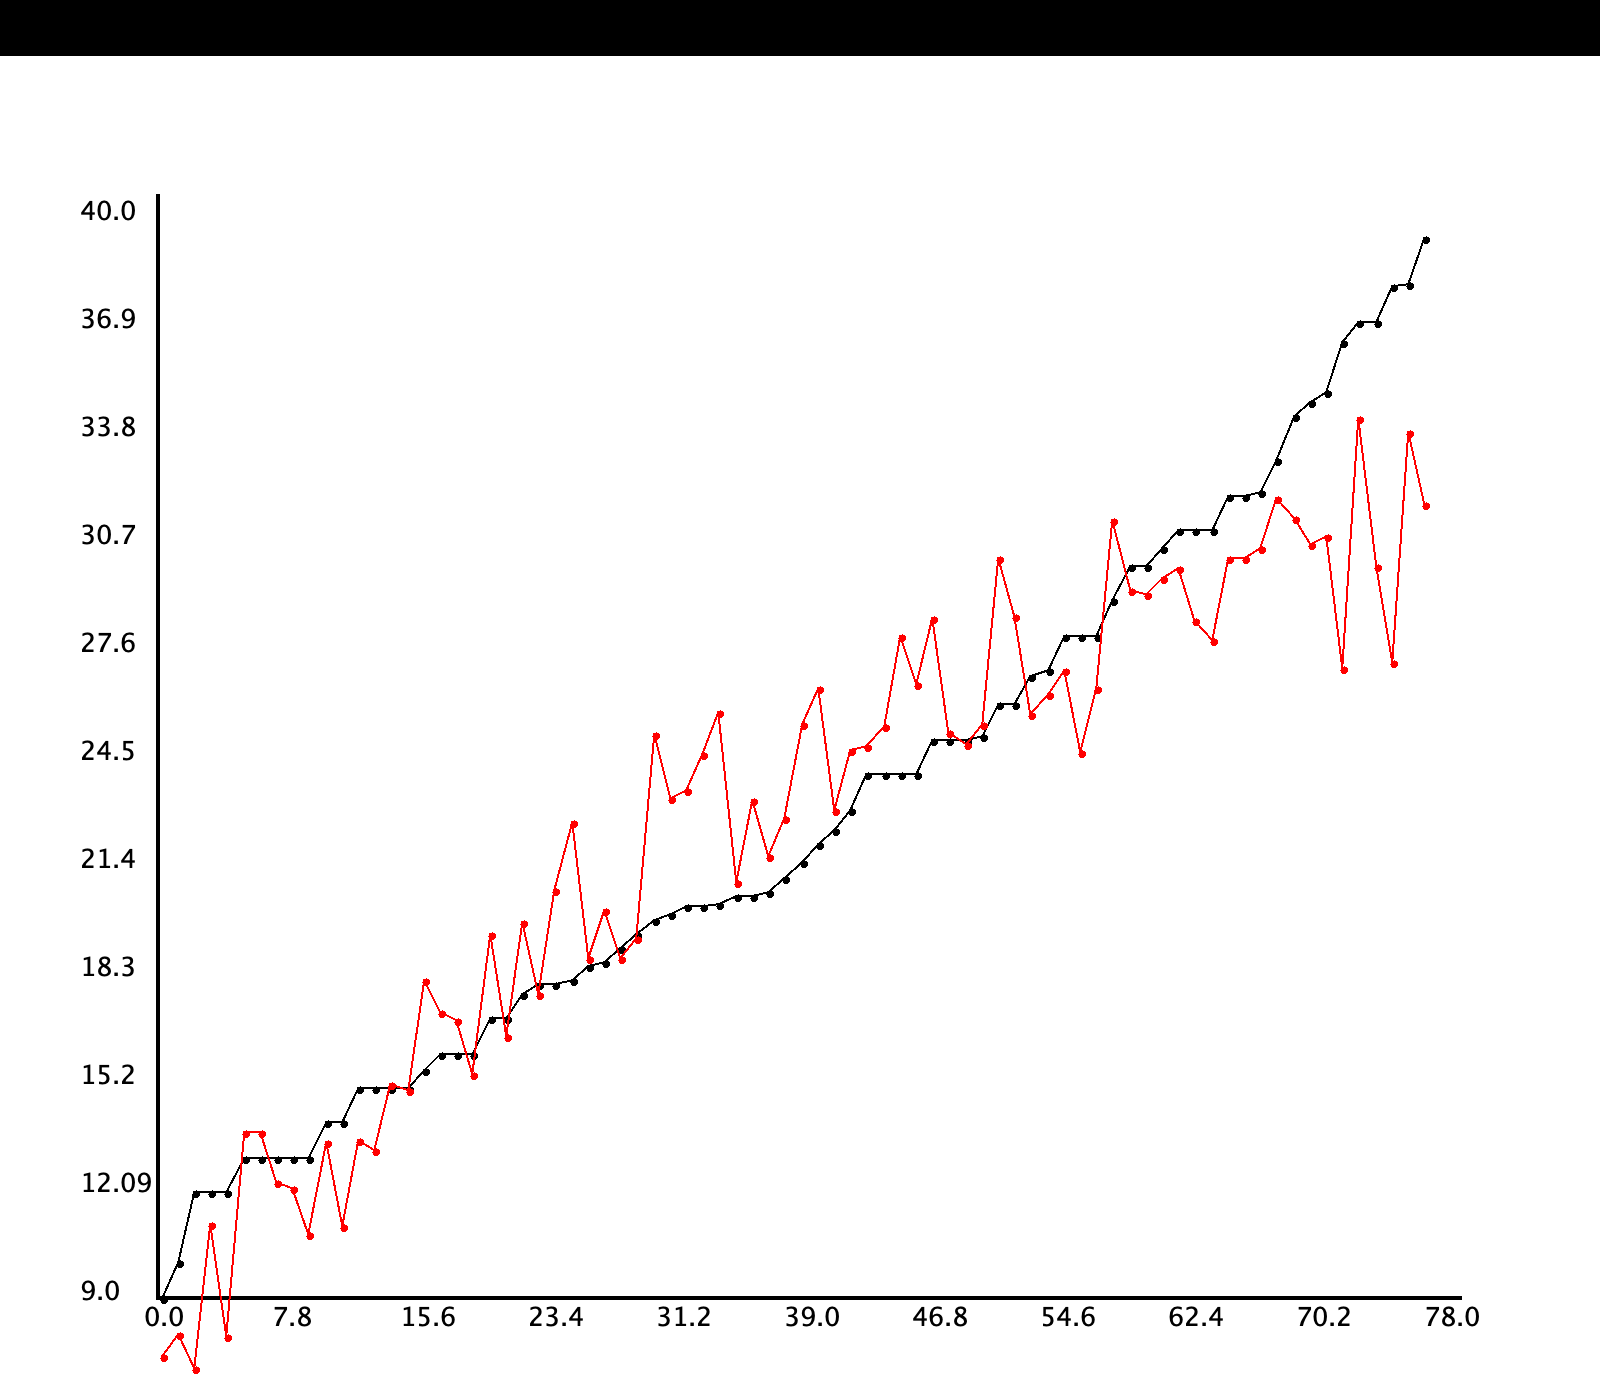
\includegraphics[width=\textwidth]{../Auto_MPG_P2/Scalation_2L_80_20.png}
     \end{subfigure}

     \vspace{10pt} % Add some vertical spacing between rows

     % Second Row
     \begin{subfigure}[b]{0.49\textwidth}
         \centering
         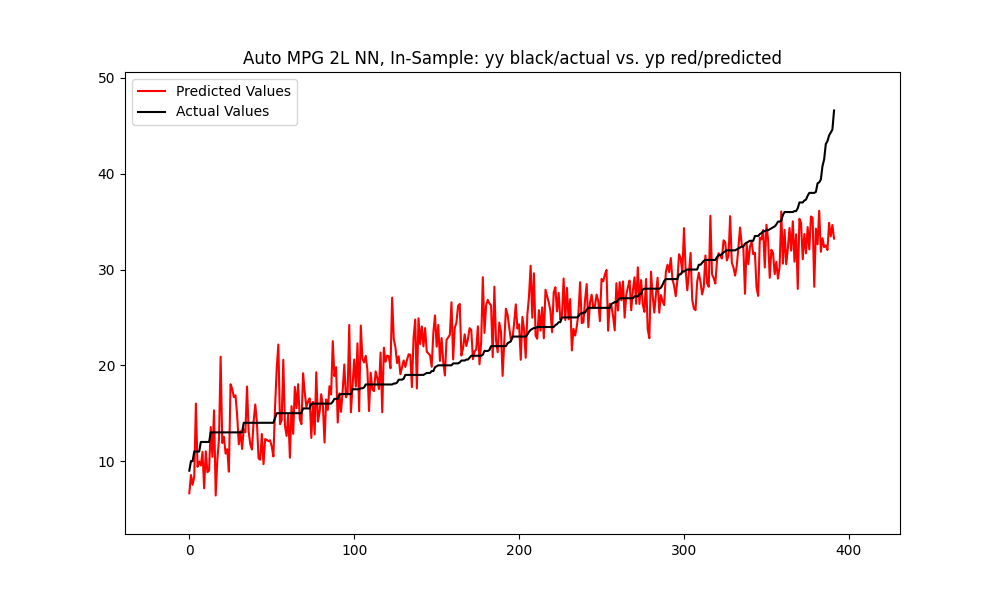
\includegraphics[width=\textwidth]{../Auto_MPG_P2/PyTorch_2L_In_Sample.png}
     \end{subfigure}
     \hfill
     \begin{subfigure}[b]{0.49\textwidth}
         \centering
         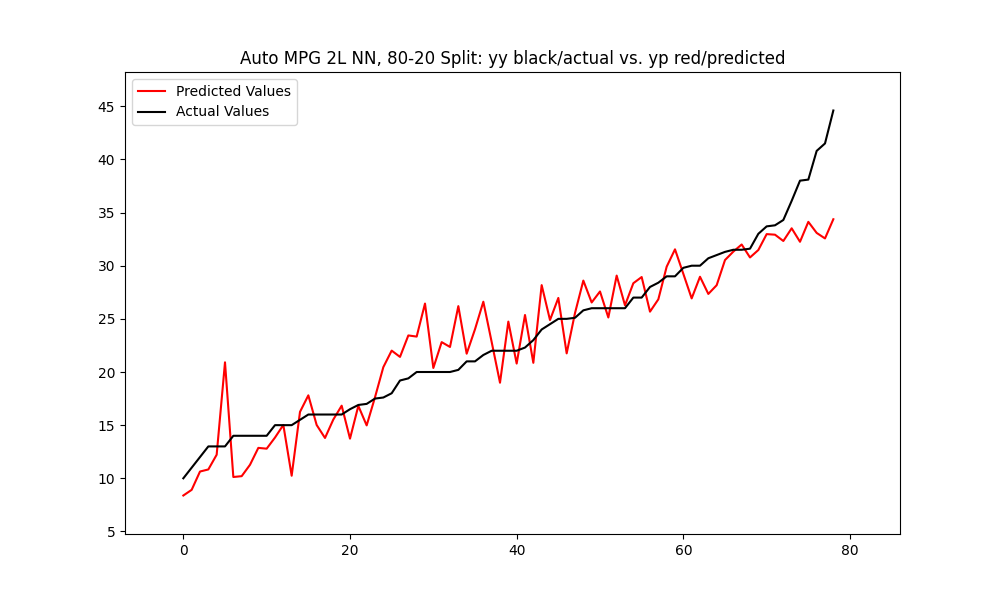
\includegraphics[width=\textwidth]{../Auto_MPG_P2/PyTorch_2L_80_20.png}
     \end{subfigure}
     
     \caption{Auto MPG 2 Layer Neural Network Plots\\ Top Left: Scalation In-Sample, Top Right: Scalation Out-of-Sample\\ Bottom Left: PyTorch In-Sample, Bottom Right: PyTorch Out-of-Sample\\ black: actual y-values, red: predicted y-values}
     \label{fig:Auto MPG 2L Plots}
\end{figure}

\subsection{3 Layer Neural Network}

In Scalation, the best results were found when using sigmoid as the activation function for the hidden layer, reLU as the activation function for the output layer, $3\times x.dim2=24$ nodes in the hidden layer, a learning rate of $0.01$, and a batch size of $8$. The results are shown in \Cref{tab:Scalation - Auto MPG 3L NN}. In PyTorch, the best results were found when using LeakyReLU as the activation function for the hidden layer, identity as the activation function for the output layer, $100$ nodes in the hidden layer, a learning rate of $0.01$, and a batch size of $32$. The results are shown in \Cref{tab:PyTorch - Auto MPG 3L NN}. Plots for In-Sample and Out-of-Sample testing can be found in \Cref{fig:Auto MPG 3L Plots}.

\begin{table}[H]
\centering
\caption{Scalation - Auto MPG 3L NN}
\label{tab:Scalation - Auto MPG 3L NN}
\begin{tabular}{|c|c|c|} \hline 
Metric & In-Sample & 80-20 Split \\ \hline \hline 
rSq &0.930275 & 0.868516 \\ \hline 
rSqBar &0.928822 &      0.865777 \\ \hline 
sst &23819.0 &  4731.23 \\ \hline 
sse &1660.78 &  622.081 \\ \hline 
sde &2.05245 &  2.79802 \\ \hline 
mse0 &4.23669 & 7.97540 \\ \hline 
rmse &2.05832 & 2.82407 \\ \hline 
mae &1.50903 &  2.03520 \\ \hline 
smape &6.54887 &        8.62759 \\ \hline 
m &392.000 &    78.0000 \\ \hline 
dfr &8.00000 &  8.00000 \\ \hline 
df &384.000 &   384.000 \\ \hline 
fStat &640.418 &        317.064 \\ \hline 
aic &-821.212 & -173.675 \\ \hline 
bic &-785.471 & -152.464 \\ \hline 
\end{tabular}
\end{table}

\begin{table}[H]
\centering
\caption{PyTorch - Auto MPG 3L NN}
\label{tab:PyTorch - Auto MPG 3L NN}
\begin{tabular}{|c|c|c|}\hline
Metric & In-Sample & 80-20 Split \\ \hline \hline
rSq & 0.8855 & 0.9095 \\ \hline
rSqBar & 0.8835 & 0.9005 \\ \hline
sst & 23818.9935 & 4910.2699 \\ \hline
sse & 2726.1212 & 444.5322 \\ \hline
sde & 2.6644 & 2.5022 \\ \hline
mse0 & 6.9544 & 5.6270 \\ \hline
rmse & 2.6371 & 2.3721 \\ \hline
mae & 1.8997 & 1.6043 \\ \hline
smape & 8.0857 & 7.0419 \\ \hline
m & 392.0000 & 79.0000 \\ \hline
dfr & 8.0000 & 8.0000 \\ \hline
df & 384.0000 & 71.0000 \\ \hline
fStat & 371.3914 & 89.1576 \\ \hline
aic & 776.2343 & 152.4784 \\ \hline
bic & 808.0044 & 171.4340 \\ \hline
\end{tabular}
\end{table}

\begin{figure}[H]
     \centering
     \captionsetup{justification=centering}
     % First Row
     \begin{subfigure}[b]{0.4\textwidth}
         \centering
         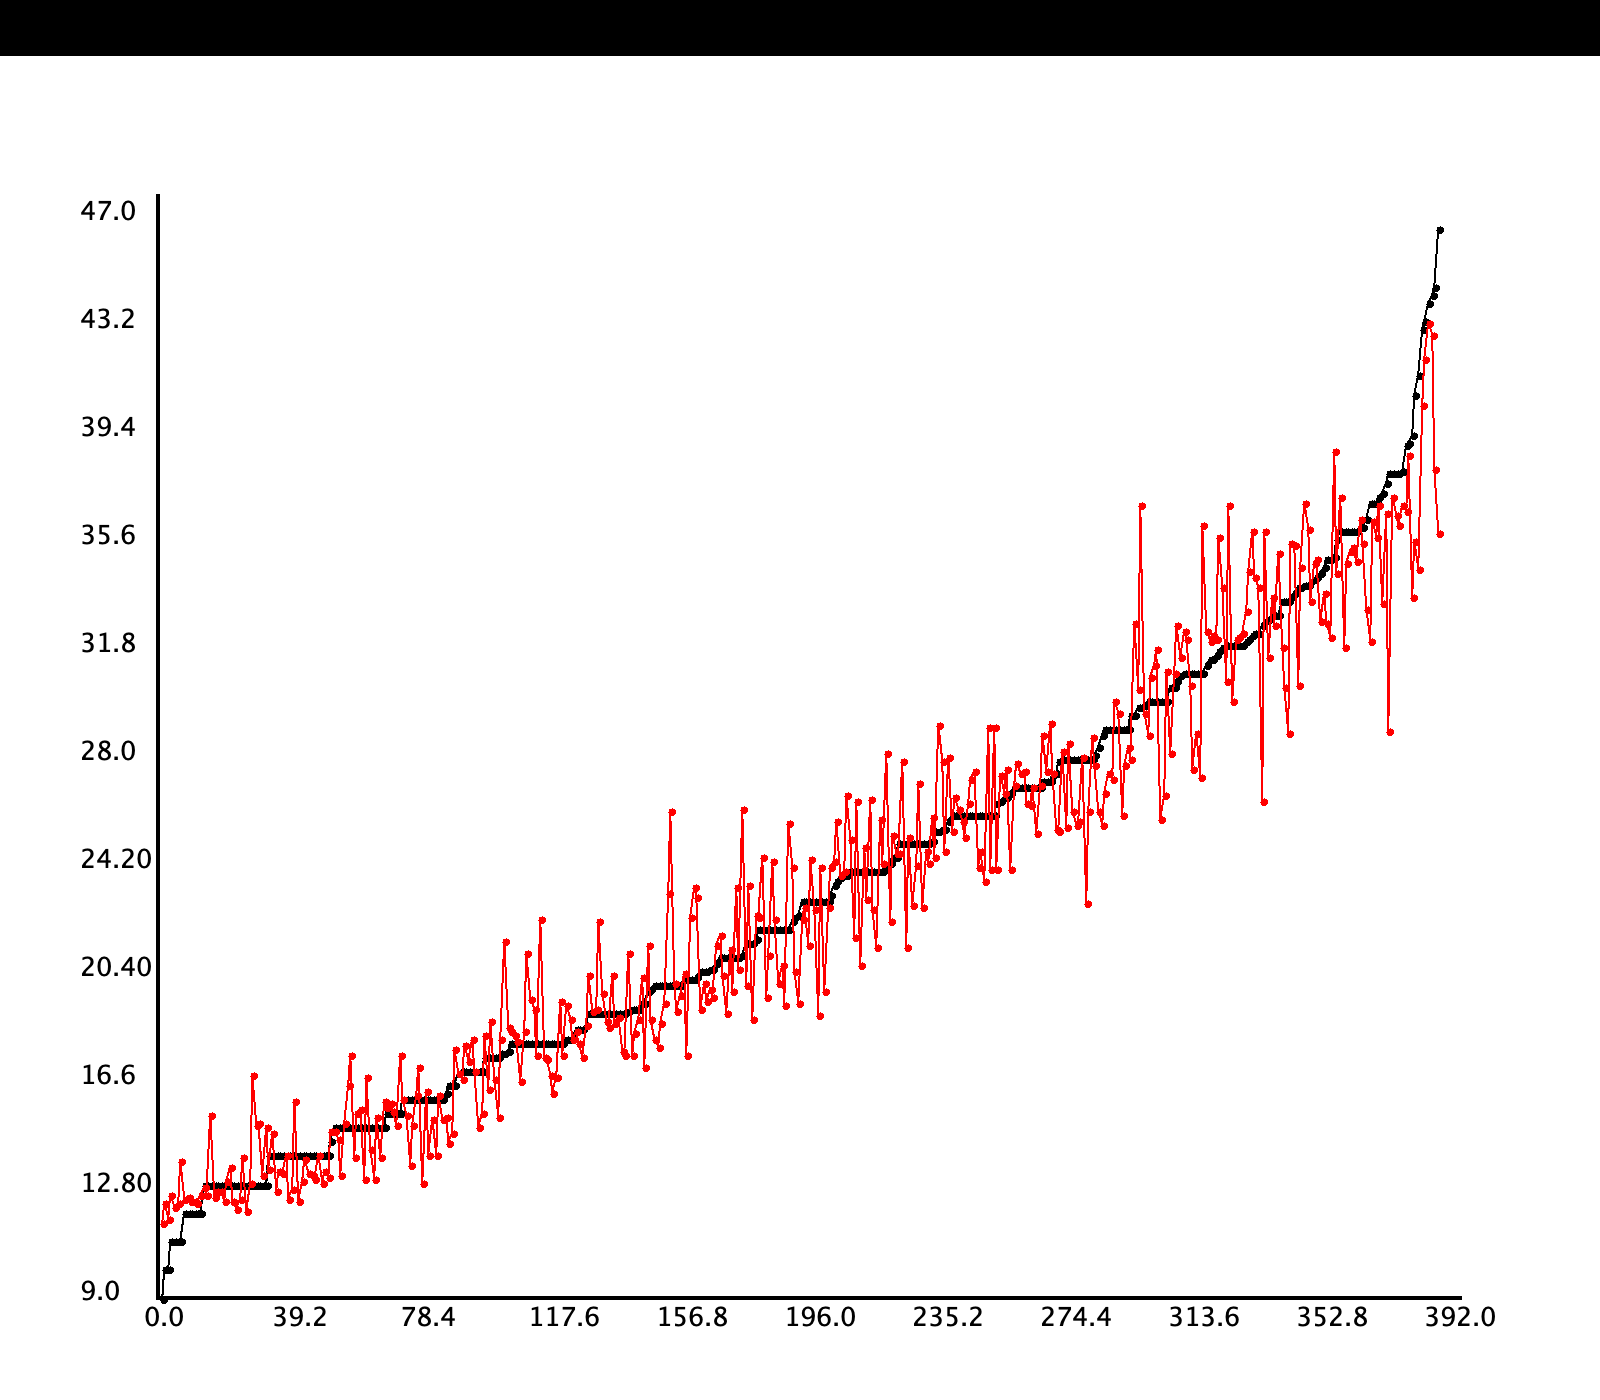
\includegraphics[width=\textwidth]{../Auto_MPG_P2/Scalation_3L_In_Sample.png}
     \end{subfigure}
     \hfill
     \begin{subfigure}[b]{0.4\textwidth}
         \centering
         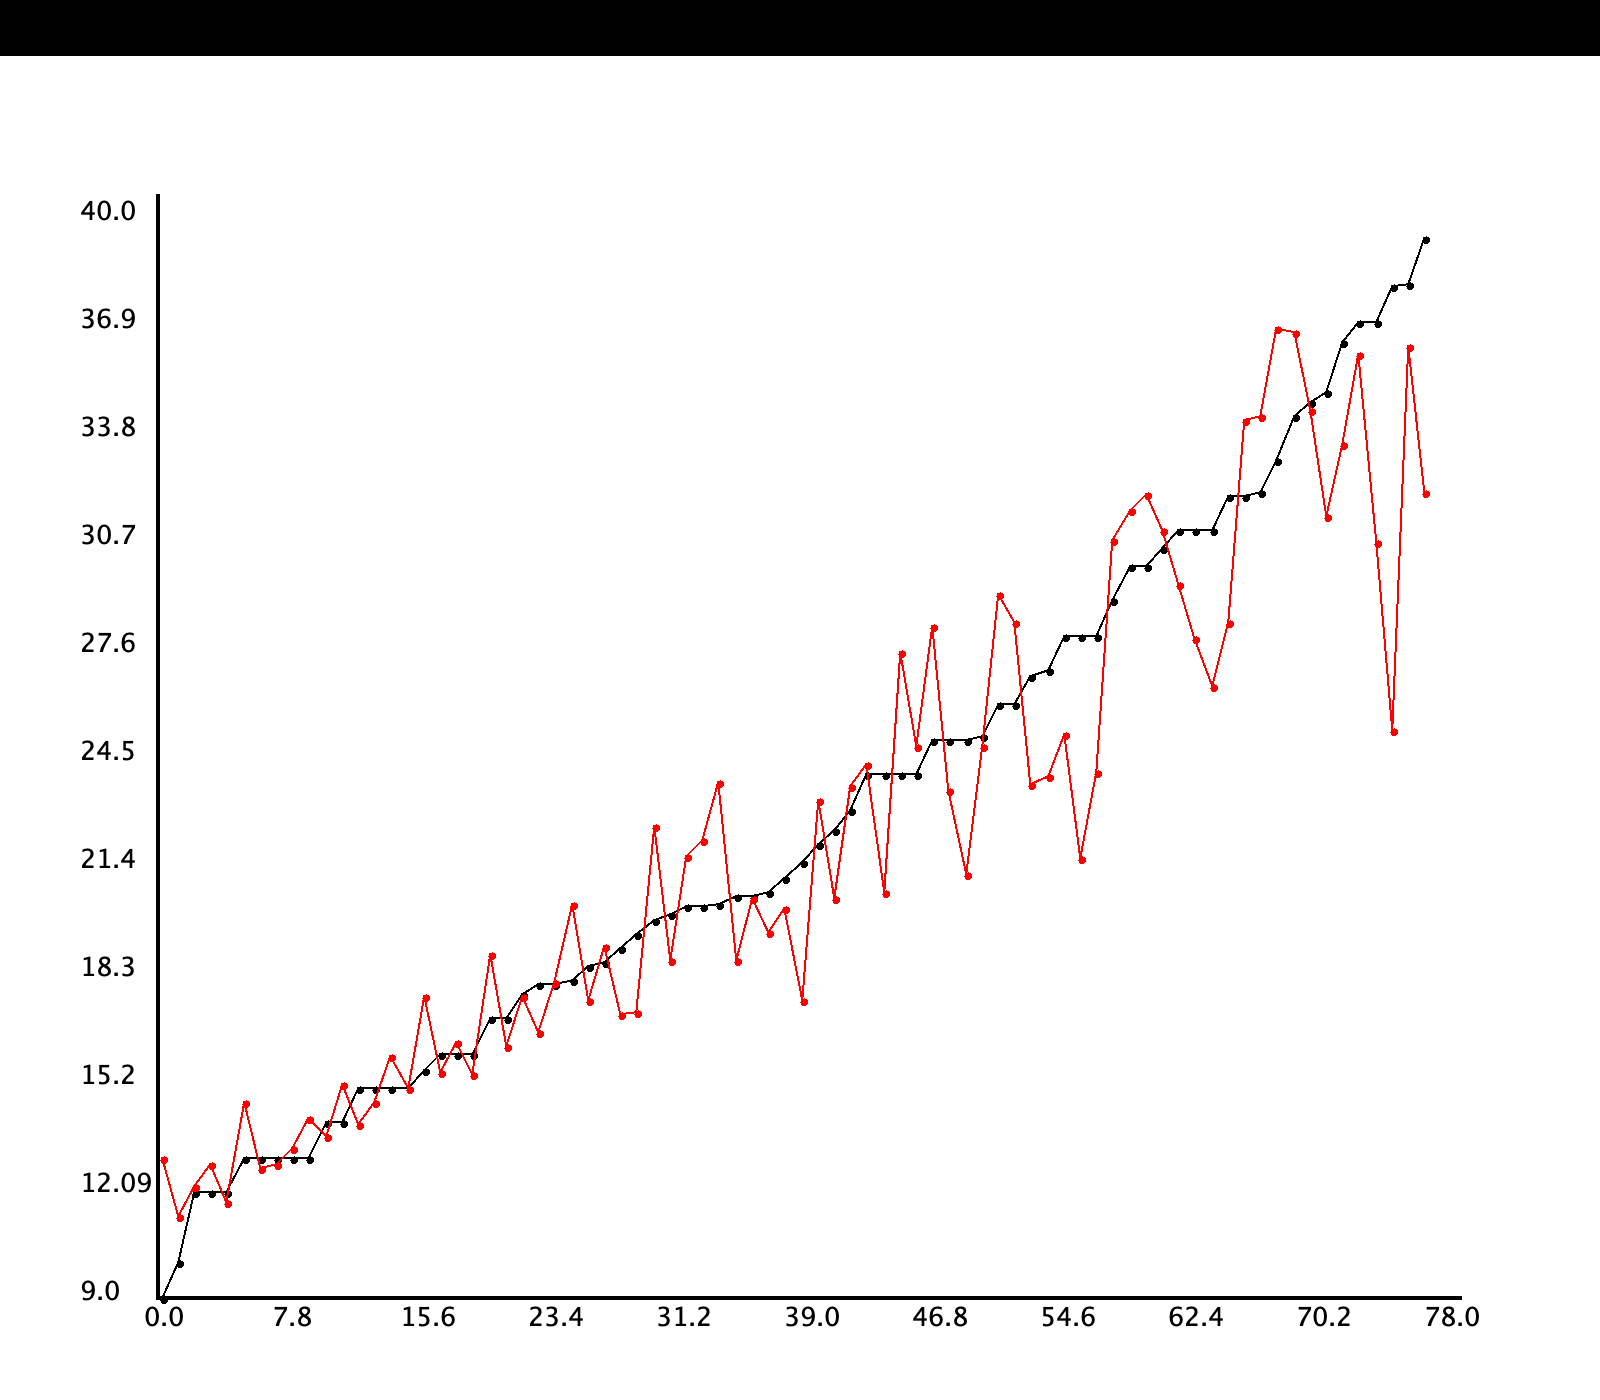
\includegraphics[width=\textwidth]{../Auto_MPG_P2/Scalation_3L_80_20.png}
     \end{subfigure}

     \vspace{10pt} % Add some vertical spacing between rows

     % Second Row
     \begin{subfigure}[b]{0.49\textwidth}
         \centering
         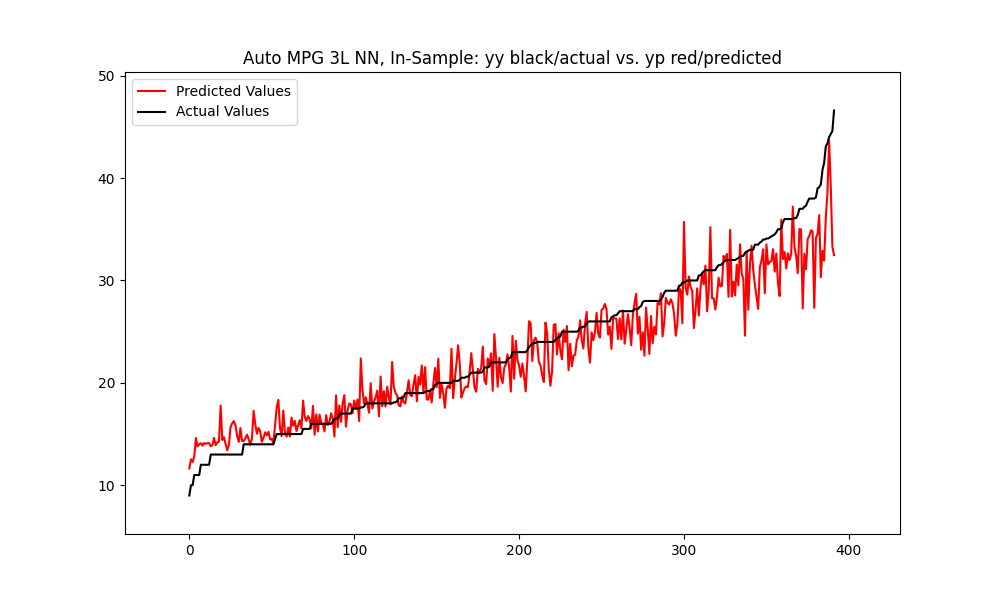
\includegraphics[width=\textwidth]{../Auto_MPG_P2/PyTorch_3L_In_Sample.png}
     \end{subfigure}
     \hfill
     \begin{subfigure}[b]{0.49\textwidth}
         \centering
         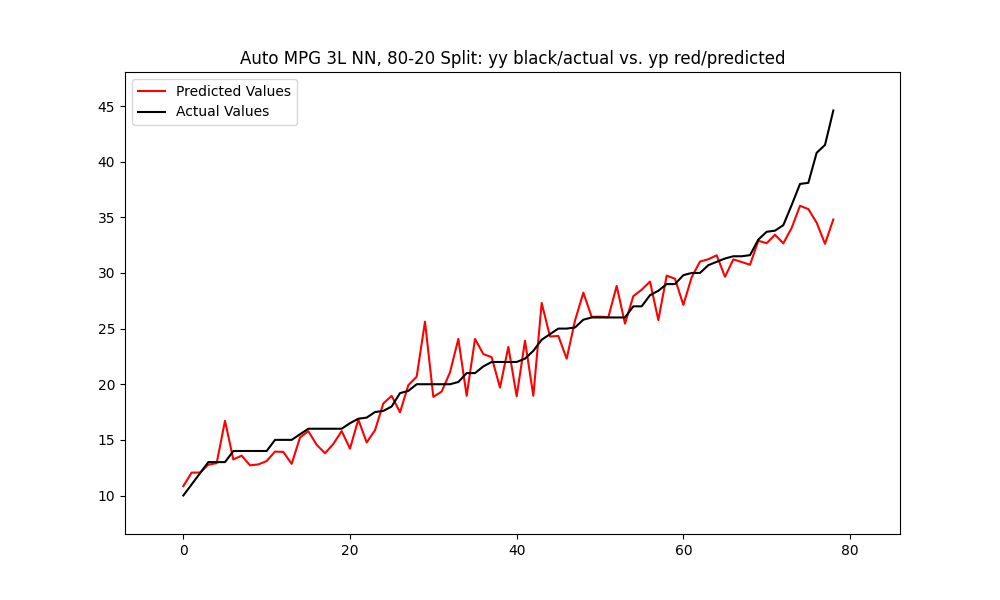
\includegraphics[width=\textwidth]{../Auto_MPG_P2/PyTorch_3L_80_20.png}
     \end{subfigure}
     
     \caption{Auto MPG 3 Layer Neural Network Plots\\ Top Left: Scalation In-Sample, Top Right: Scalation Out-of-Sample\\ Bottom Left: PyTorch In-Sample, Bottom Right: PyTorch Out-of-Sample\\ black: actual y-values, red: predicted y-values}
     \label{fig:Auto MPG 3L Plots}
\end{figure}

\subsection{4 Layer Neural Network}

\section{California House Prices}

\subsection{2 Layer Neural Network}

In Scalation, the best results were found when using the reLU as the activation function, a learning rate of $25$, and a batch size of $32$. We note the unusually high learning rate that was required in order to get good results. This is most likely due to the y-values having a large scale. The results are shown in \Cref{tab:Scalation - California House Prices 2L NN}. In PyTorch, the best results were found when using the reLU as the activation function, a learning rate of $0.01$, and a batch size of $32$. The results are shown in \Cref{tab:PyTorch - California House Prices 2L NN}. Plots for In-Sample and Out-of-Sample testing can be found in \Cref{fig:California House Prices 2L Plots}.

\begin{table}[H]
\centering
\caption{Scalation - California House Prices 2L NN}
\label{tab:Scalation - California House Prices 2L NN}
\begin{tabular}{|c|c|c|} \hline 
Metric & In-Sample & 80-20 Split \\ \hline \hline 
rSq &0.633776 & 0.630655 \\ \hline 
rSqBar &0.633579 &      0.630456 \\ \hline 
sst &2.72264e+14 &      5.31945e+13 \\ \hline 
sse &9.97097e+13 &      1.96471e+13 \\ \hline 
sde &69653.2 &  69346.2 \\ \hline 
mse0 &4.87984e+09 &     4.80840e+09 \\ \hline 
rmse &69855.8 & 69342.6 \\ \hline 
mae &51821.3 &  50737.2 \\ \hline 
smape &26.8854 &        26.5678 \\ \hline 
m &20433.0 &    4086.00 \\ \hline 
dfr &11.0000 &  11.0000 \\ \hline 
df &20421.0 &   20421.0 \\ \hline 
fStat &3212.73 &        3169.89 \\ \hline 
aic &-256883 &  -51319.7 \\ \hline 
bic &-256788 &  -51243.9 \\ \hline 
\end{tabular}
\end{table}

\begin{table}[H]
\centering
\caption{PyTorch - California House Prices 2L NN}
\label{tab:PyTorch - California House Prices 2L NN}
\begin{tabular}{|c|c|c|}\hline
Metric & In-Sample & 80-20 Split \\ \hline \hline
rSq & 0.6468 & 0.6516 \\ \hline
rSqBar & 0.6466 & 0.6506 \\ \hline
sst & 272264434648930.1875 & 54723646809444.8438 \\ \hline
sse & 96172625731084.4375 & 19066274074331.2266 \\ \hline
sde & 68625.7706 & 68402.0487 \\ \hline
mse0 & 4706730569.7198 & 4665102538.3732 \\ \hline
rmse & 68605.6162 & 68301.5559 \\ \hline
mae & 49654.9430 & 50131.4253 \\ \hline
smape & 26.7647 & 26.6343 \\ \hline
m & 20433.0000 & 4087.0000 \\ \hline
dfr & 12.0000 & 12.0000 \\ \hline
df & 20421.0000 & 4075.0000 \\ \hline
fStat & 3115.8995 & 635.0821 \\ \hline
aic & 455113.0754 & 91014.4163 \\ \hline
bic & 455208.1743 & 91090.2031 \\ \hline
\end{tabular}
\end{table}

\begin{figure}[H]
     \centering
     \captionsetup{justification=centering}
     % First Row
     \begin{subfigure}[b]{0.4\textwidth}
         \centering
         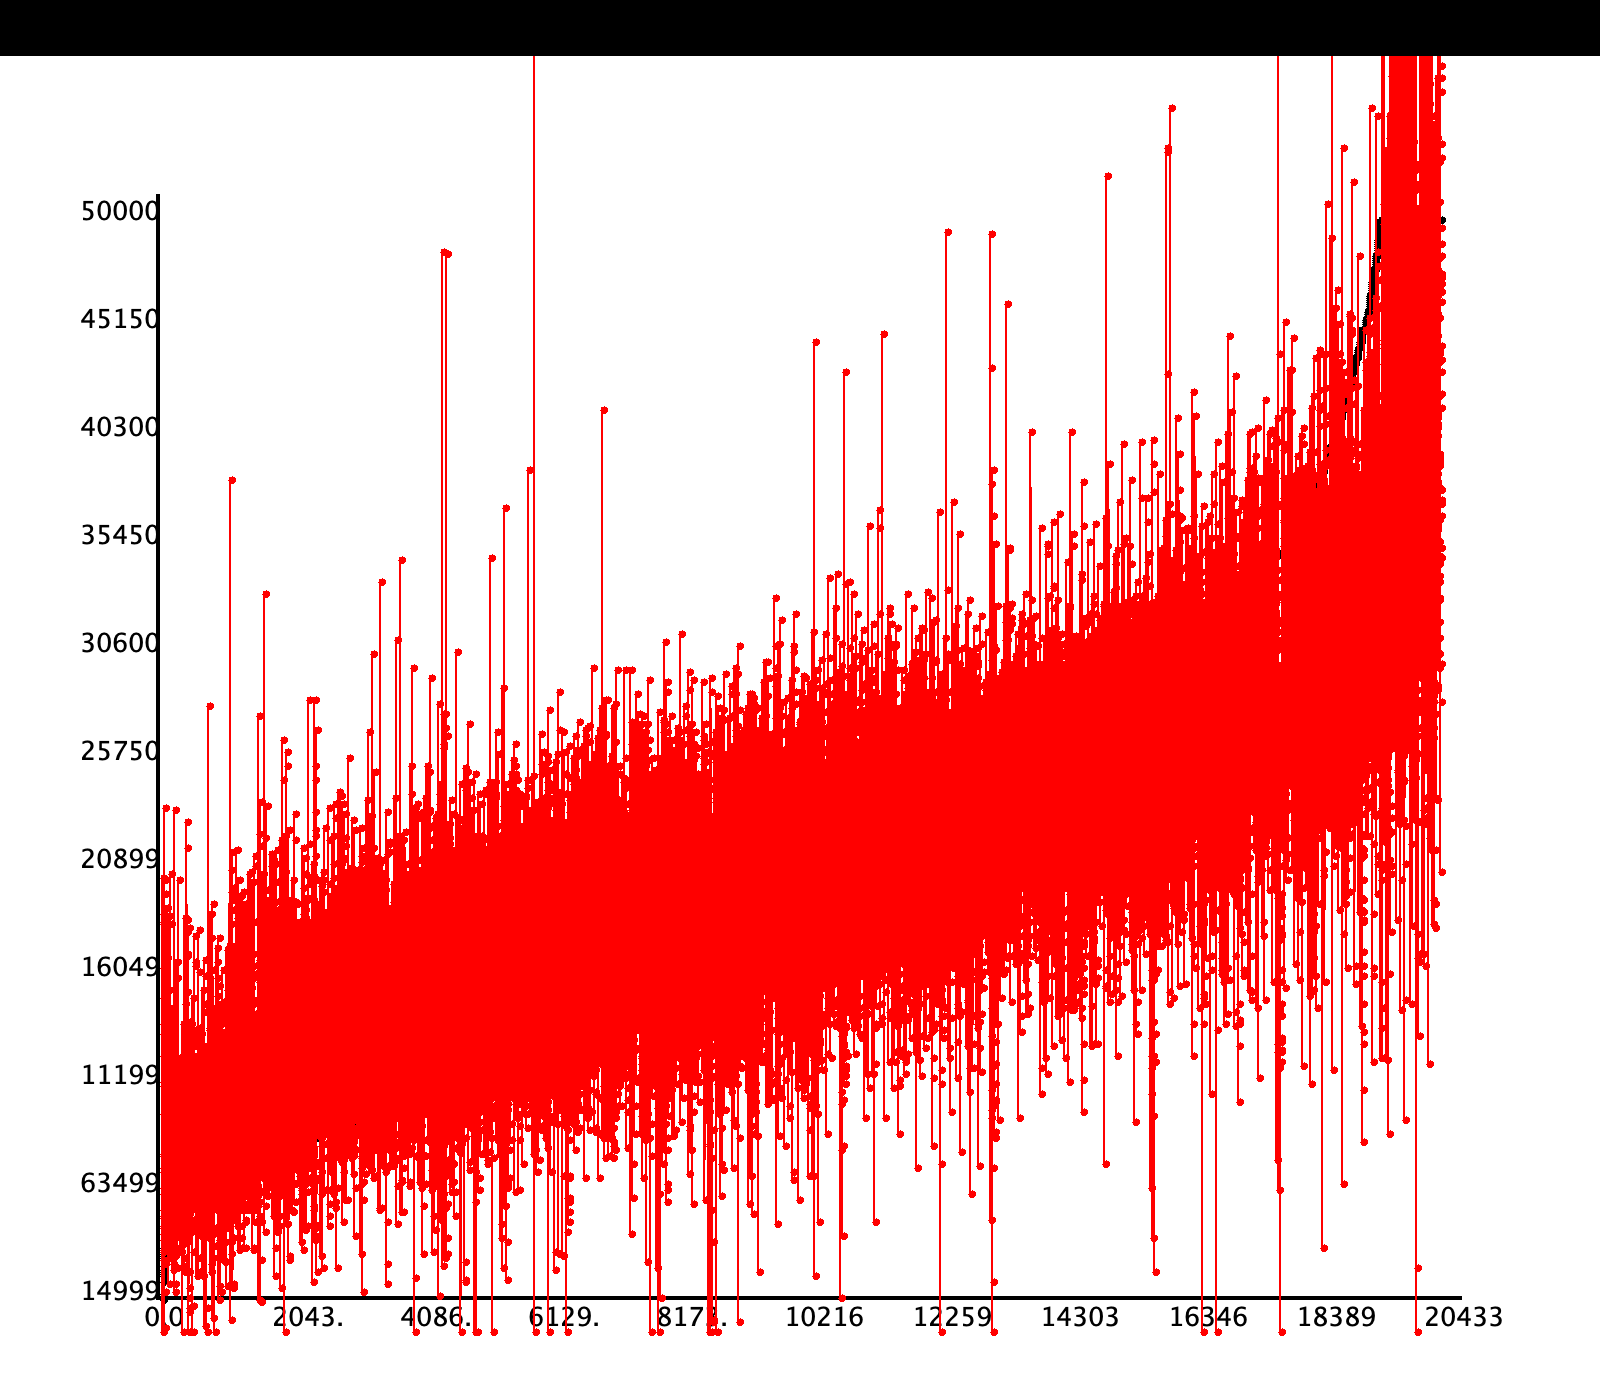
\includegraphics[width=\textwidth]{../Housing_P2/Scalation_2L_In_Sample.png}
     \end{subfigure}
     \hfill
     \begin{subfigure}[b]{0.4\textwidth}
         \centering
         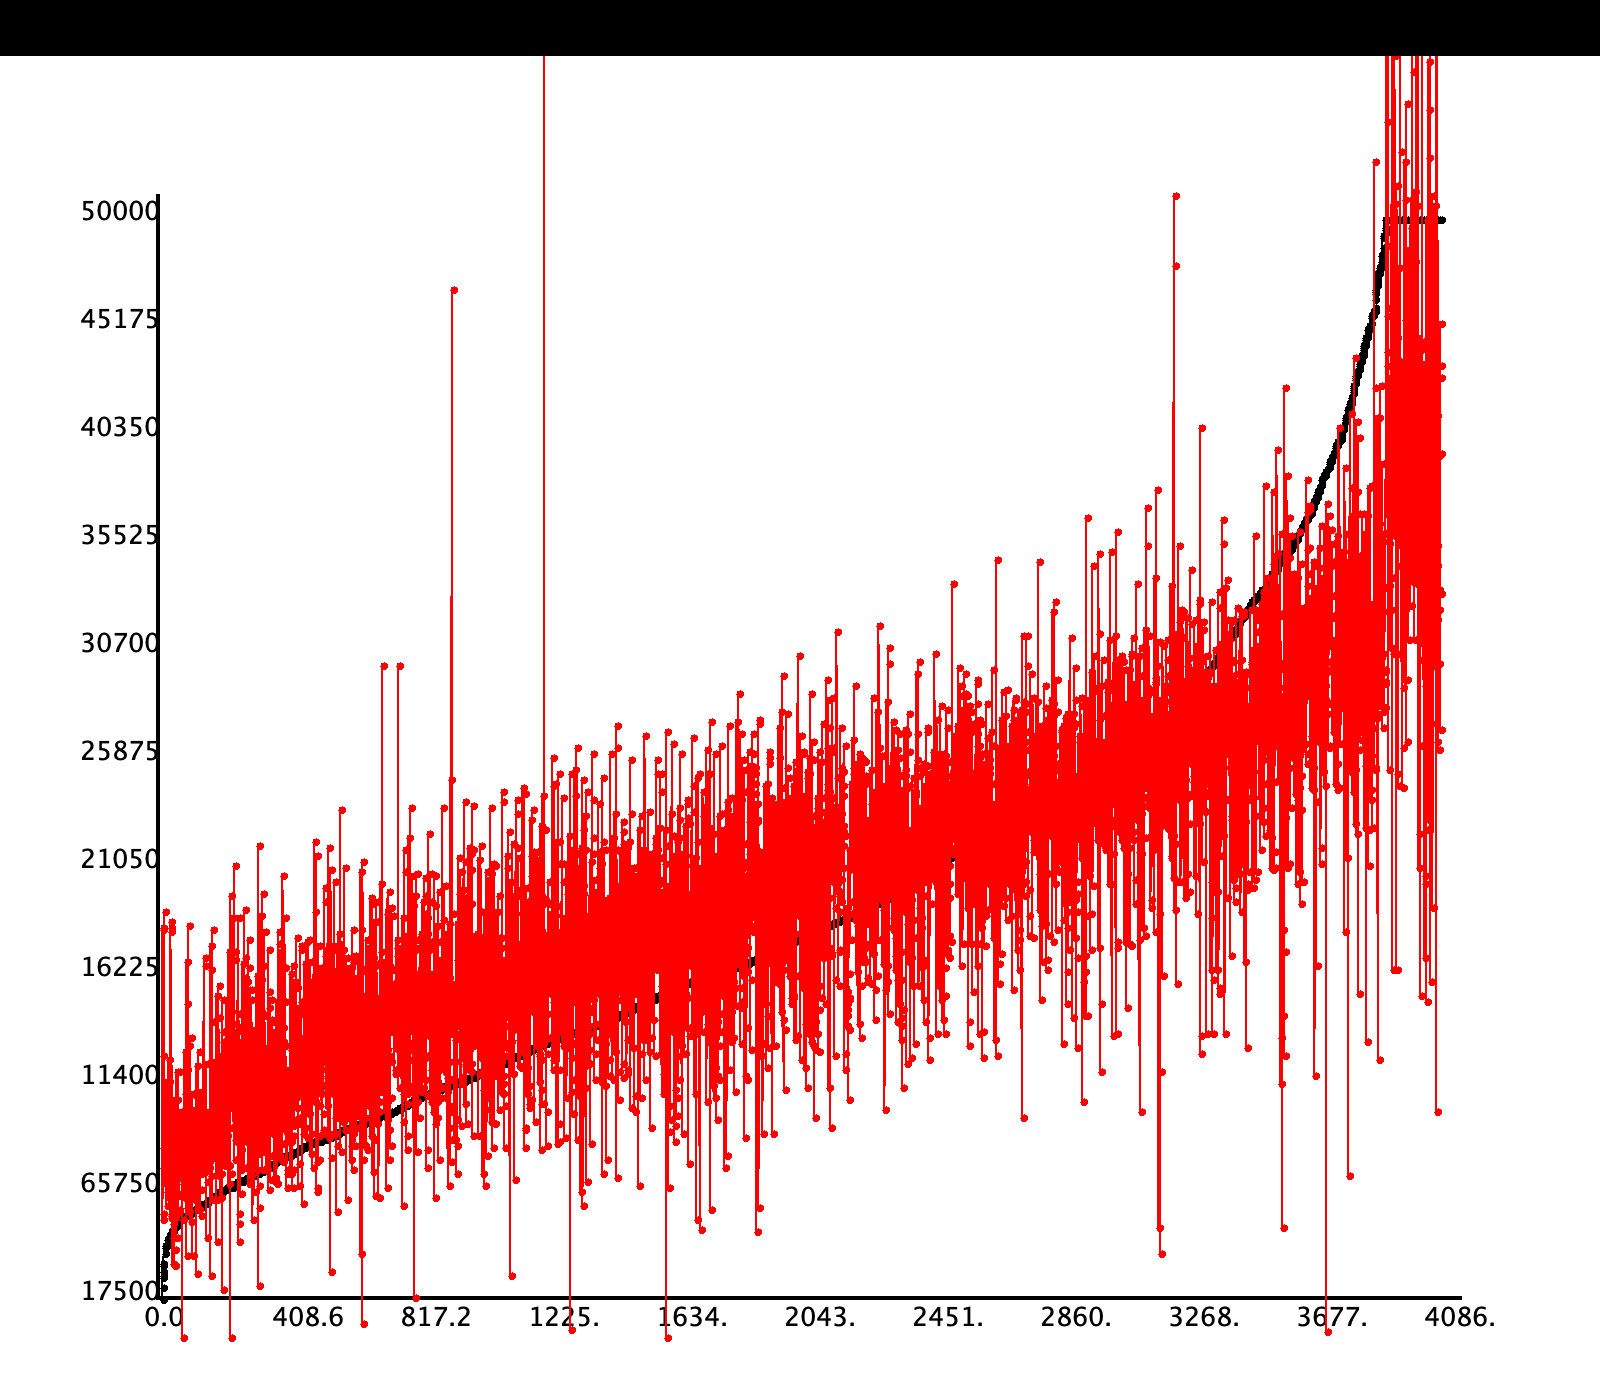
\includegraphics[width=\textwidth]{../Housing_P2/Scalation_2L_80_20.png}
     \end{subfigure}

     \vspace{10pt} % Add some vertical spacing between rows

     % Second Row
     \begin{subfigure}[b]{0.49\textwidth}
         \centering
         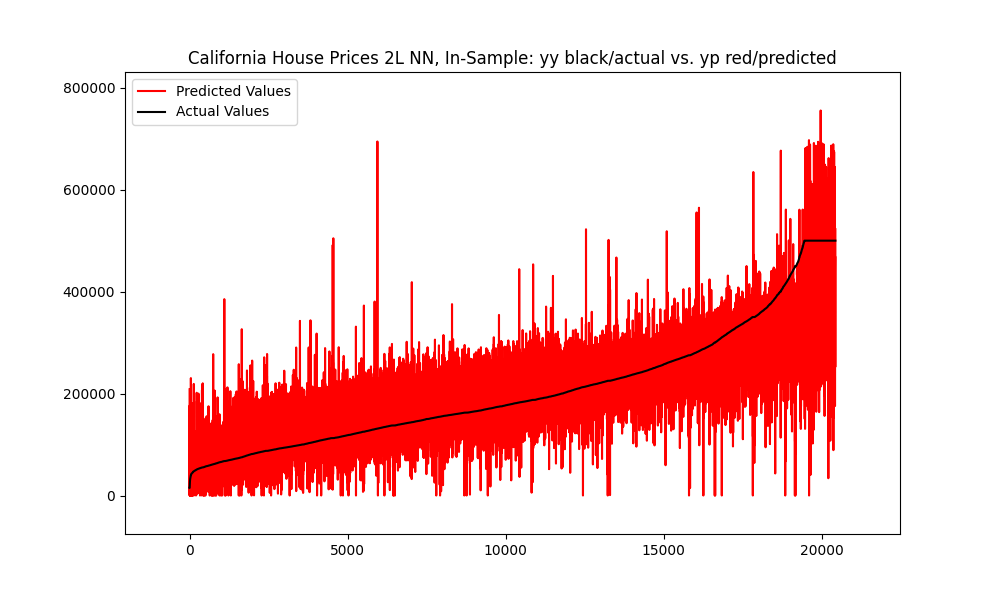
\includegraphics[width=\textwidth]{../Housing_P2/PyTorch_2L_In_Sample.png}
     \end{subfigure}
     \hfill
     \begin{subfigure}[b]{0.49\textwidth}
         \centering
         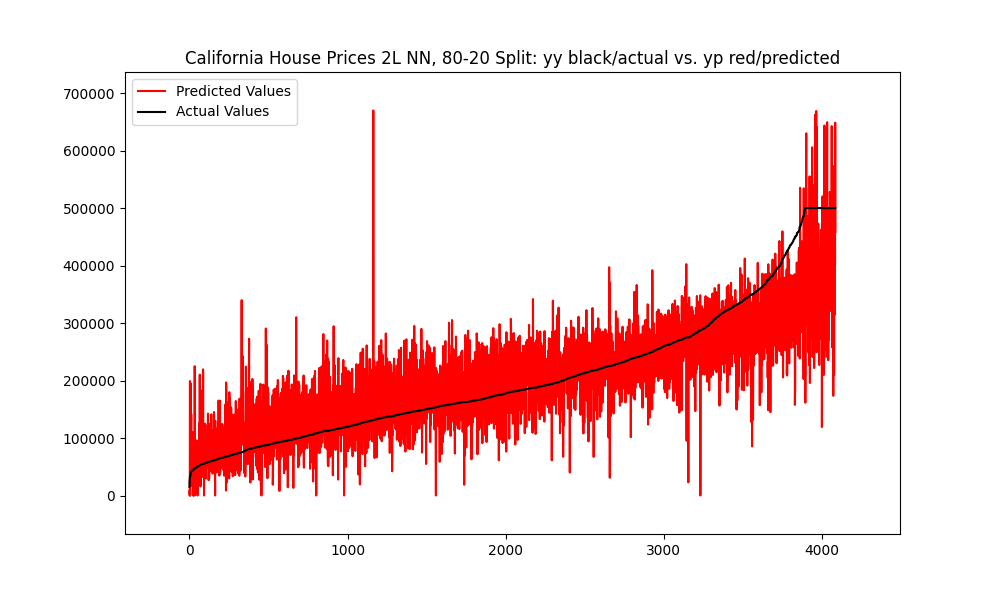
\includegraphics[width=\textwidth]{../Housing_P2/PyTorch_2L_80_20.png}
     \end{subfigure}
     
     \caption{California House Prices 2 Layer Neural Network Plots\\ Top Left: Scalation In-Sample, Top Right: Scalation Out-of-Sample\\ Bottom Left: PyTorch In-Sample, Bottom Right: PyTorch Out-of-Sample\\ black: actual y-values, red: predicted y-values}
     \label{fig:California House Prices 2L Plots}
\end{figure}

\subsection{3 Layer Neural Network}

In Scalation, the best results were found when using lreLU as the activation function for the hidden layer, identity as the activation function for the output layer, $3\times x.dim2=36$ nodes in the hidden layer, a learning rate of $0.01$, and a batch size of $32$. The results are shown in \Cref{tab:Scalation - California House Prices 3L NN}. In PyTorch, the best results were found when using LeakyReLU as the activation function for the hidden layer, identity as the activation function for the output layer, $100$ nodes in the hidden layer, a learning rate of $0.01$, and a batch size of $32$. The results are shown in \Cref{tab:PyTorch - California House Prices 3L NN}. Plots for In-Sample and Out-of-Sample testing can be found in \Cref{fig:California House Prices 3L Plots}.

\begin{table}[H]
\centering
\caption{Scalation - California House Prices 3L NN}
\label{tab:Scalation - California House Prices 3L NN}
\begin{tabular}{|c|c|c|} \hline 
Metric & In-Sample & 80-20 Split \\ \hline \hline 
rSq &0.779769 & 0.756155 \\ \hline 
rSqBar &0.779639 &      0.756012 \\ \hline 
sst &27226.4 &  5319.45 \\ \hline 
sse &5996.11 &  1297.12 \\ \hline 
sde &0.541323 & 0.562612 \\ \hline 
mse0 &0.293452 &        0.317454 \\ \hline 
rmse &0.541712 &        0.563431 \\ \hline 
mae &0.371532 & 0.389204 \\ \hline 
smape &19.3019 &        20.5293 \\ \hline 
m &20433.0 &    4086.00 \\ \hline 
dfr &12.0000 &  12.0000 \\ \hline 
df &20421.0 &   20421.0 \\ \hline 
fStat &6025.36 &        5277.08 \\ \hline 
aic &-16441.3 & -3427.61 \\ \hline 
bic &-16338.3 & -3345.51 \\ \hline 
\end{tabular}
\end{table}

\begin{table}[H]
\centering
\caption{PyTorch - California House Prices 3L NN}
\label{tab:PyTorch - California House Prices 3L NN}
\begin{tabular}{|c|c|c|}\hline
Metric & In-Sample & 80-20 Split \\ \hline \hline
rSq & 0.8057 & 0.7961 \\ \hline
rSqBar & 0.8056 & 0.7956 \\ \hline
sst & 272264434648930.1250 & 54723646809444.8281 \\ \hline
sse & 52901444882088.6094 & 11156430483920.8633 \\ \hline
sde & 50897.3609 & 52323.7456 \\ \hline
mse0 & 2589019961.9287 & 2729735865.8970 \\ \hline
rmse & 50882.4131 & 52246.8742 \\ \hline
mae & 34838.6035 & 35574.6590 \\ \hline
smape & 18.1115 & 18.1492 \\ \hline
m & 20433.0000 & 4087.0000 \\ \hline
dfr & 12.0000 & 12.0000 \\ \hline
df & 20421.0000 & 4075.0000 \\ \hline
fStat & 7056.5363 & 1326.1142 \\ \hline
aic & 442899.9831 & 88824.1727 \\ \hline
bic & 442995.0819 & 88899.9595 \\ \hline
\end{tabular}
\end{table}

\begin{figure}[H]
     \centering
     \captionsetup{justification=centering}
     % First Row
     \begin{subfigure}[b]{0.4\textwidth}
         \centering
         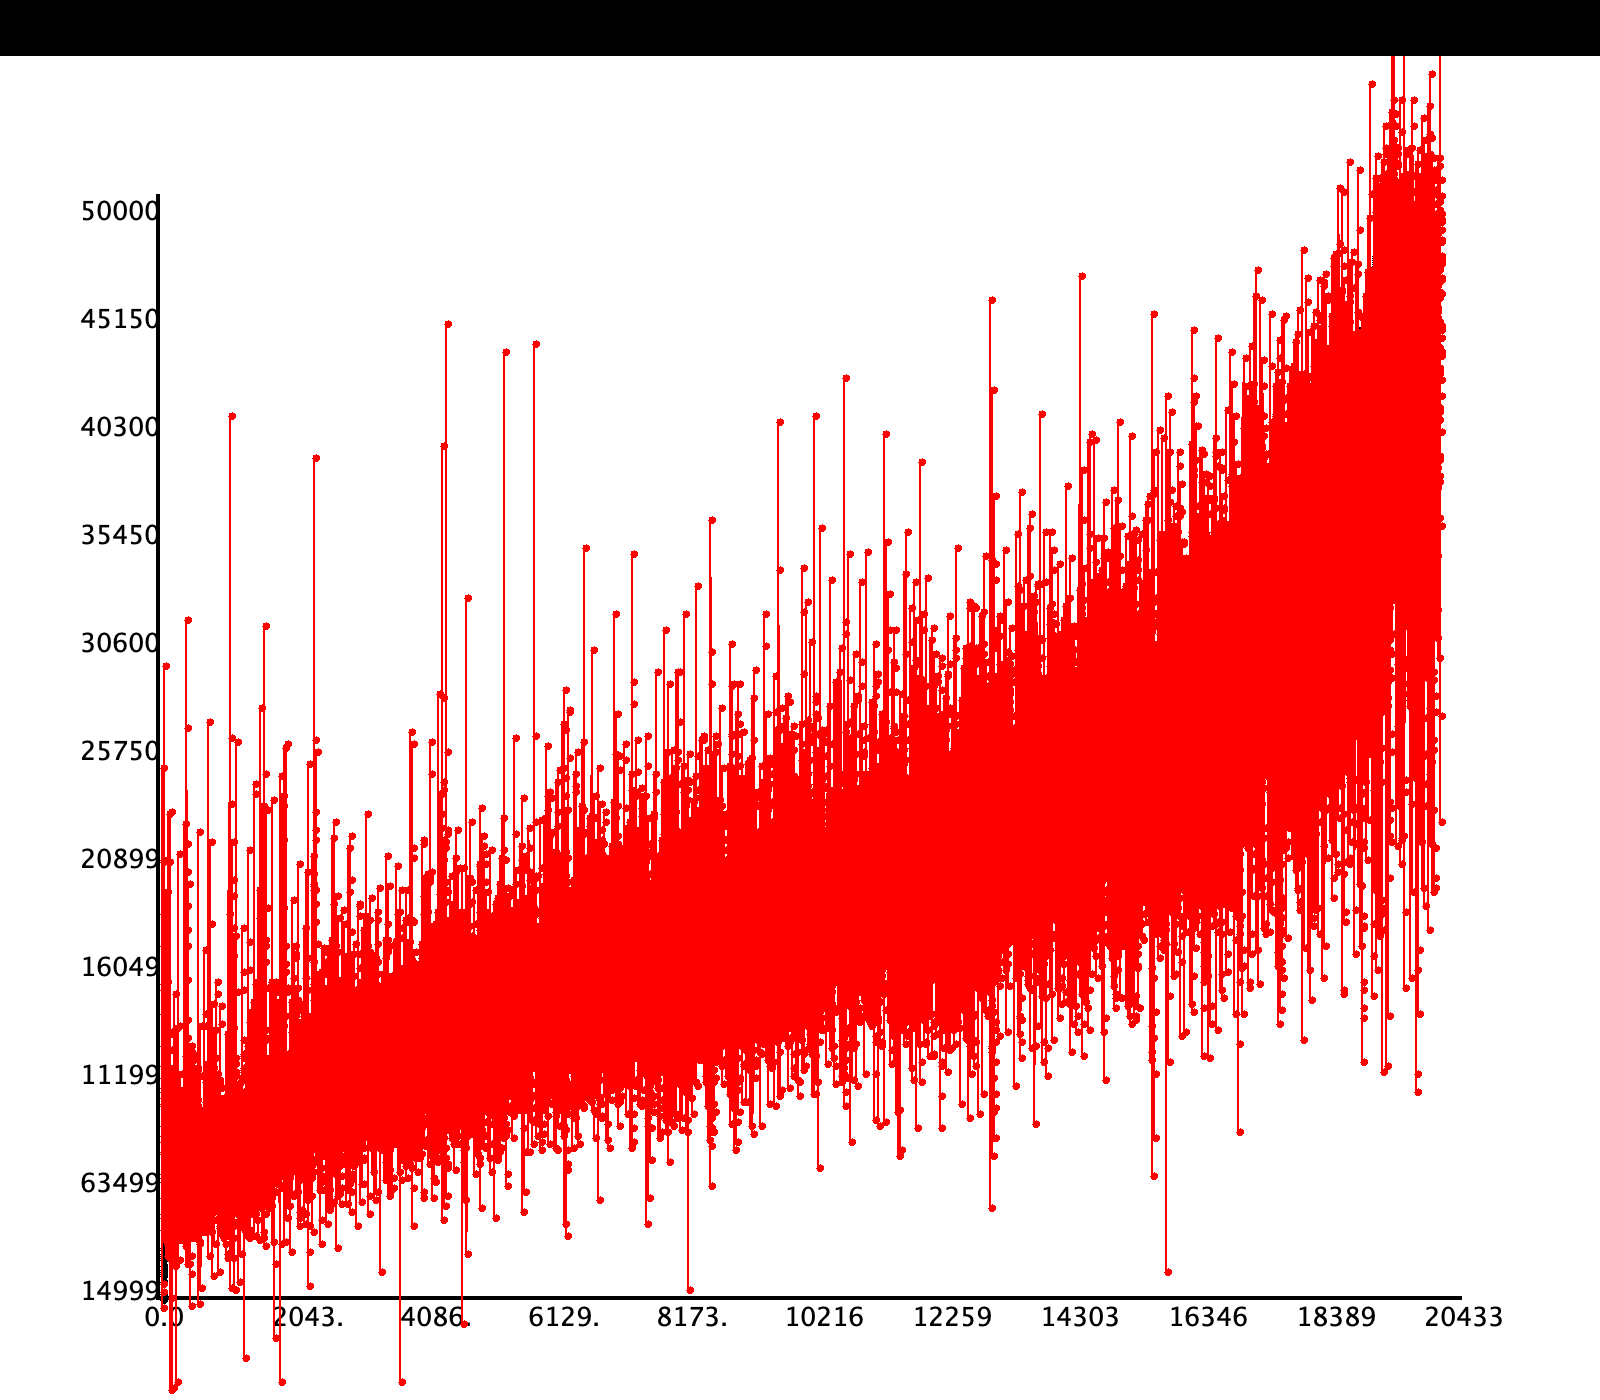
\includegraphics[width=\textwidth]{../Housing_P2/Scalation_3L_In_Sample.png}
     \end{subfigure}
     \hfill
     \begin{subfigure}[b]{0.4\textwidth}
         \centering
         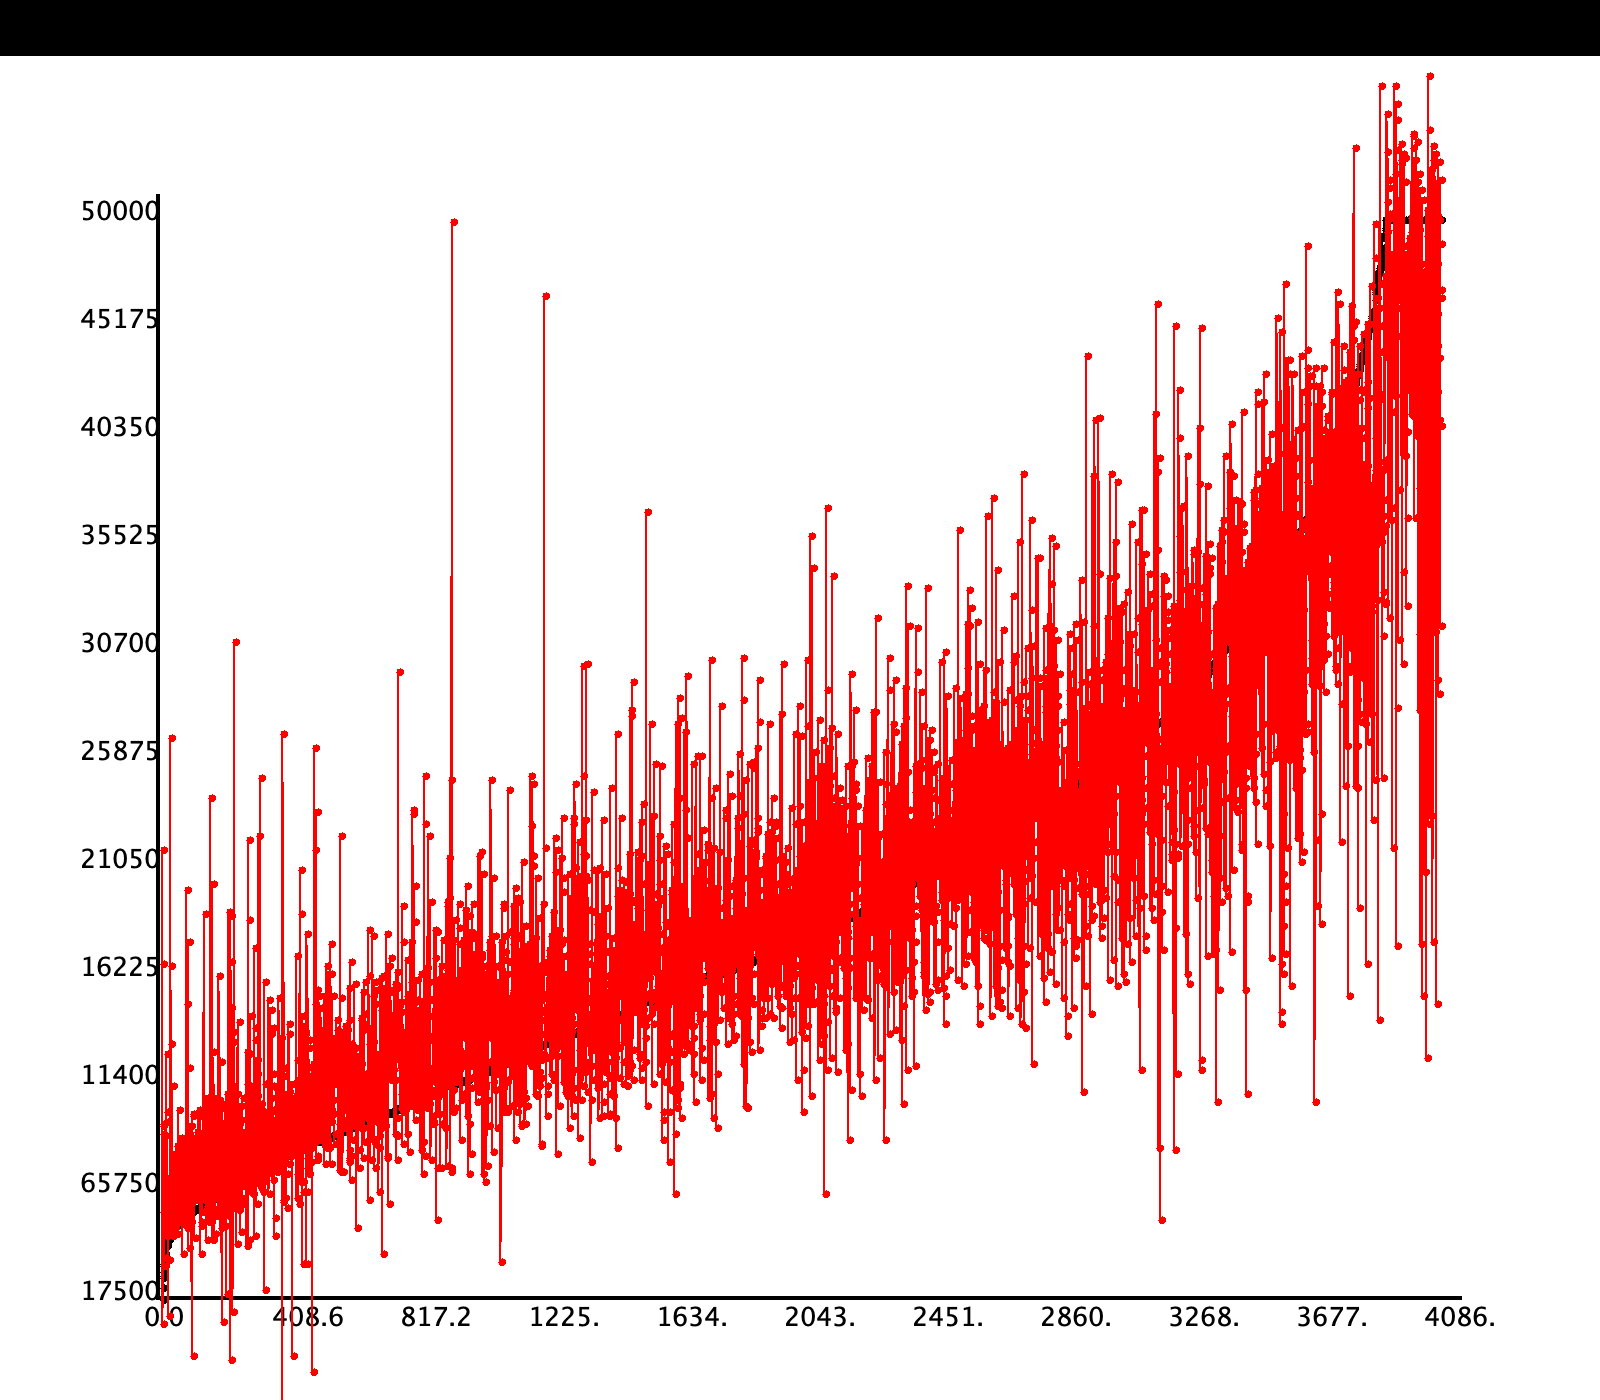
\includegraphics[width=\textwidth]{../Housing_P2/Scalation_3L_80_20.png}
     \end{subfigure}

     \vspace{10pt} % Add some vertical spacing between rows

     % Second Row
     \begin{subfigure}[b]{0.49\textwidth}
         \centering
         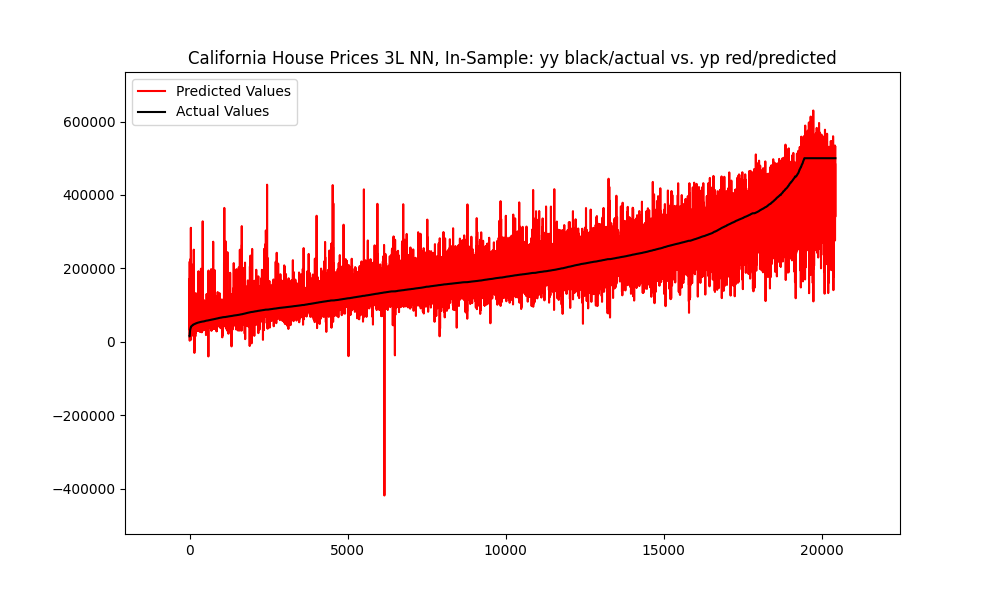
\includegraphics[width=\textwidth]{../Housing_P2/PyTorch_3L_In_Sample.png}
     \end{subfigure}
     \hfill
     \begin{subfigure}[b]{0.49\textwidth}
         \centering
         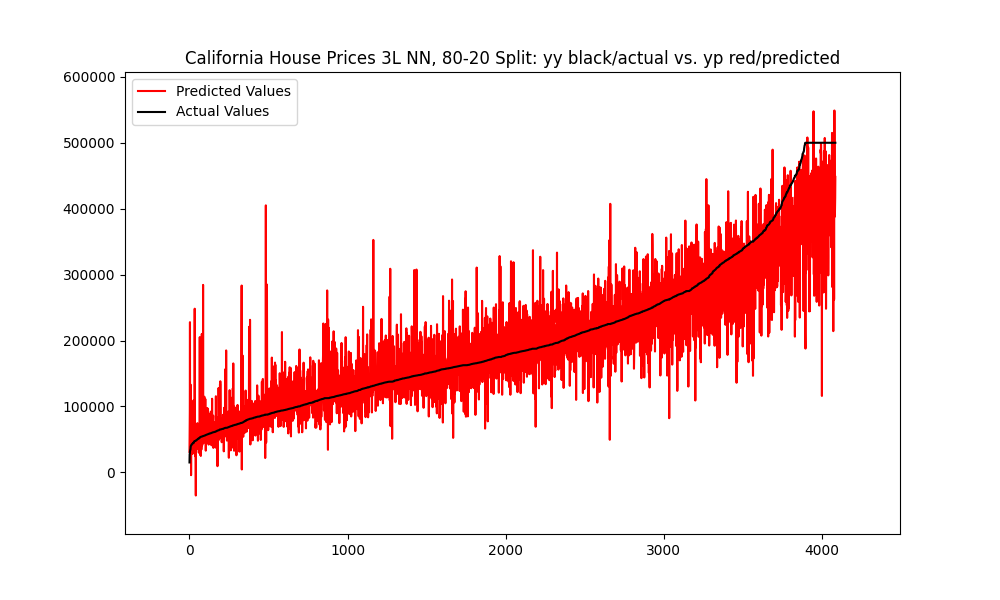
\includegraphics[width=\textwidth]{../Housing_P2/PyTorch_3L_80_20.png}
     \end{subfigure}
     
     \caption{California House Prices 3 Layer Neural Network Plots\\ Top Left: Scalation In-Sample, Top Right: Scalation Out-of-Sample\\ Bottom Left: PyTorch In-Sample, Bottom Right: PyTorch Out-of-Sample\\ black: actual y-values, red: predicted y-values}
     \label{fig:California House Prices 3L Plots}
\end{figure}

\subsection{4 Layer Neural Network}

\section{Insurance Charges}

\subsection{2 Layer Neural Network}

In Scalation, the best results were found when using the reLU as the activation function, a learning rate of $200$, and a batch size of $32$. We note the unusually high learning rate that was required in order to get good results. This is most likely due to the y-values having a large scale. The results are shown in \Cref{tab:Scalation - Insurance Charges 2L NN}. In PyTorch, the best results were found when using the reLU as the activation function, a learning rate of $0.01$, and a batch size of $32$. The results are shown in \Cref{tab:PyTorch - Insurance Charges 2L NN}. Plots for In-Sample and Out-of-Sample testing can be found in \Cref{fig:Insurance Charges 2L Plots}.

\begin{table}[H]
\centering
\caption{Scalation - Insurance Charges 2L NN}
\label{tab:Scalation - Insurance Charges 2L NN}
\begin{tabular}{|c|c|c|} \hline 
Metric & In-Sample & 80-20 Split \\ \hline \hline 
rSq &0.722979 & 0.682065 \\ \hline 
rSqBar &0.721521 &      0.680392 \\ \hline 
sst &1.96074e+11 &      4.06432e+10 \\ \hline 
sse &5.43167e+10 &      1.29219e+10 \\ \hline 
sde &6346.14 &  6966.63 \\ \hline 
mse0 &4.05954e+07 &     4.83965e+07 \\ \hline 
rmse &6371.45 & 6956.76 \\ \hline 
mae &4519.55 &  4729.99 \\ \hline 
smape &39.5992 &        41.9288 \\ \hline 
m &1338.00 &    267.000 \\ \hline 
dfr &7.00000 &  7.00000 \\ \hline 
df &1330.00 &   1330.00 \\ \hline 
fStat &495.869 &        407.607 \\ \hline 
aic &-13602.9 & -2725.13 \\ \hline 
bic &-13561.3 & -2696.43 \\ \hline 
\end{tabular}
\end{table}

\begin{table}[H]
\centering
\caption{PyTorch - Insurance Charges 2L NN}
\label{tab:PyTorch - Insurance Charges 2L NN}
\begin{tabular}{|c|c|c|}\hline
Metric & In-Sample & 80-20 Split \\ \hline \hline
rSq & 0.7516 & 0.8007 \\ \hline
rSqBar & 0.7503 & 0.7953 \\ \hline
sst & 196074221568.3671 & 42646829902.3297 \\ \hline
sse & 48702200251.0962 & 8498989265.5920 \\ \hline
sde & 6051.2970 & 5717.3788 \\ \hline
mse0 & 36399252.8035 & 31712646.5134 \\ \hline
rmse & 6033.1793 & 5631.3983 \\ \hline
mae & 4158.4738 & 3932.9280 \\ \hline
smape & 39.1264 & 36.6337 \\ \hline
m & 1338.0000 & 268.0000 \\ \hline
dfr & 8.0000 & 8.0000 \\ \hline
df & 1330.0000 & 260.0000 \\ \hline
fStat & 503.0696 & 130.5808 \\ \hline
aic & 23310.6587 & 4644.9566 \\ \hline
bic & 23352.2501 & 4673.6845 \\ \hline
\end{tabular}
\end{table}

\begin{figure}[H]
     \centering
     \captionsetup{justification=centering}
     % First Row
     \begin{subfigure}[b]{0.4\textwidth}
         \centering
         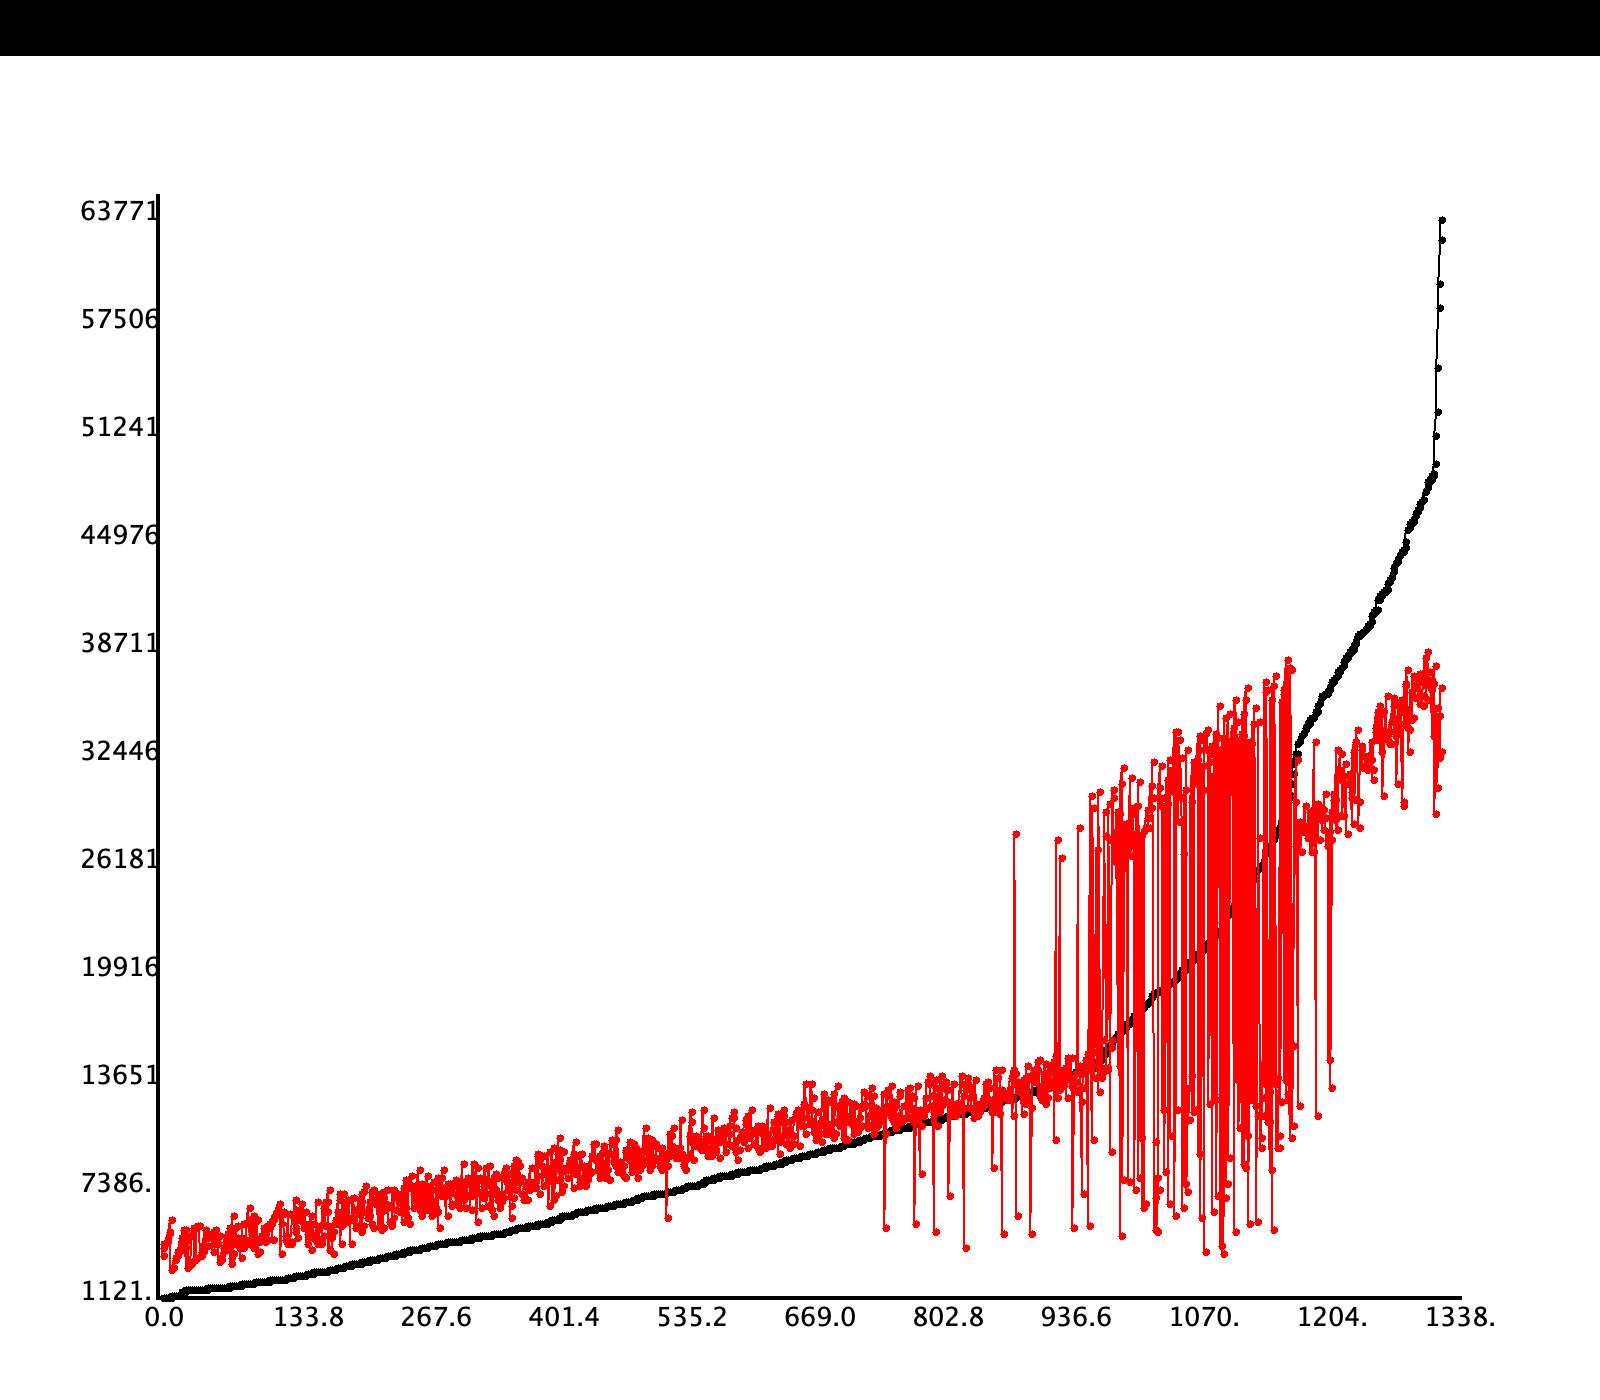
\includegraphics[width=\textwidth]{../Insurance_P2/Scalation_2L_In_Sample.png}
     \end{subfigure}
     \hfill
     \begin{subfigure}[b]{0.4\textwidth}
         \centering
         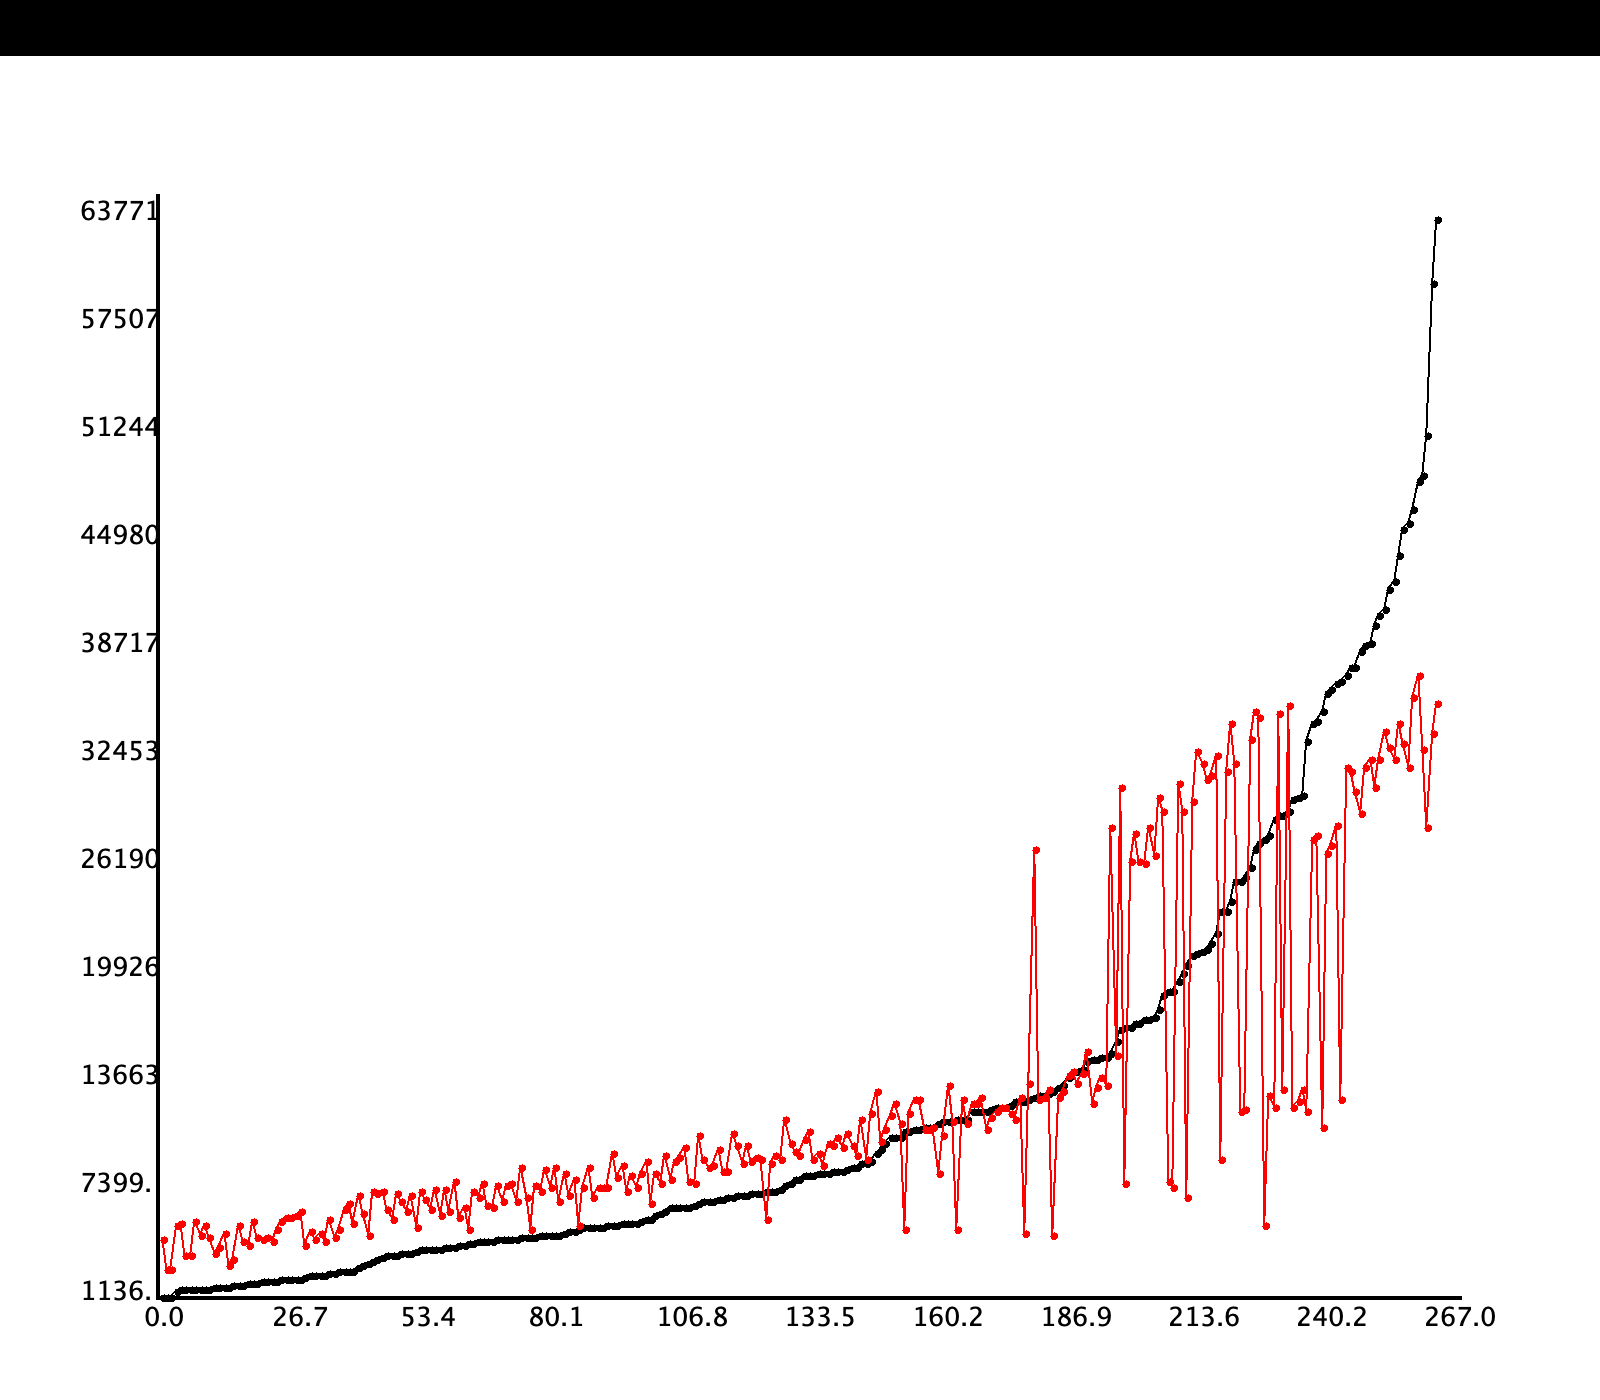
\includegraphics[width=\textwidth]{../Insurance_P2/Scalation_2L_80_20.png}
     \end{subfigure}

     \vspace{10pt} % Add some vertical spacing between rows

     % Second Row
     \begin{subfigure}[b]{0.49\textwidth}
         \centering
         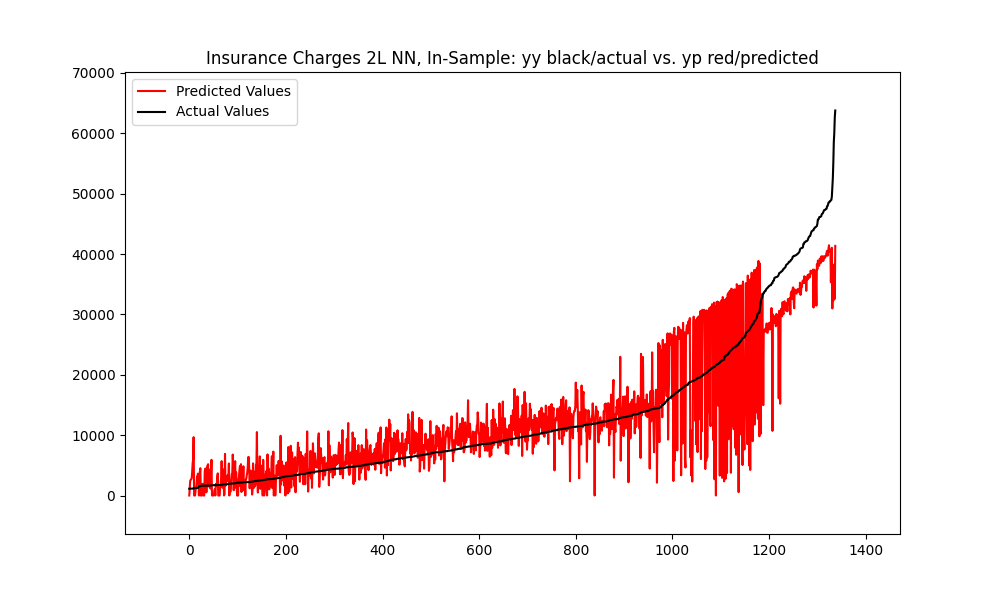
\includegraphics[width=\textwidth]{../Insurance_P2/PyTorch_2L_In_Sample.png}
     \end{subfigure}
     \hfill
     \begin{subfigure}[b]{0.49\textwidth}
         \centering
         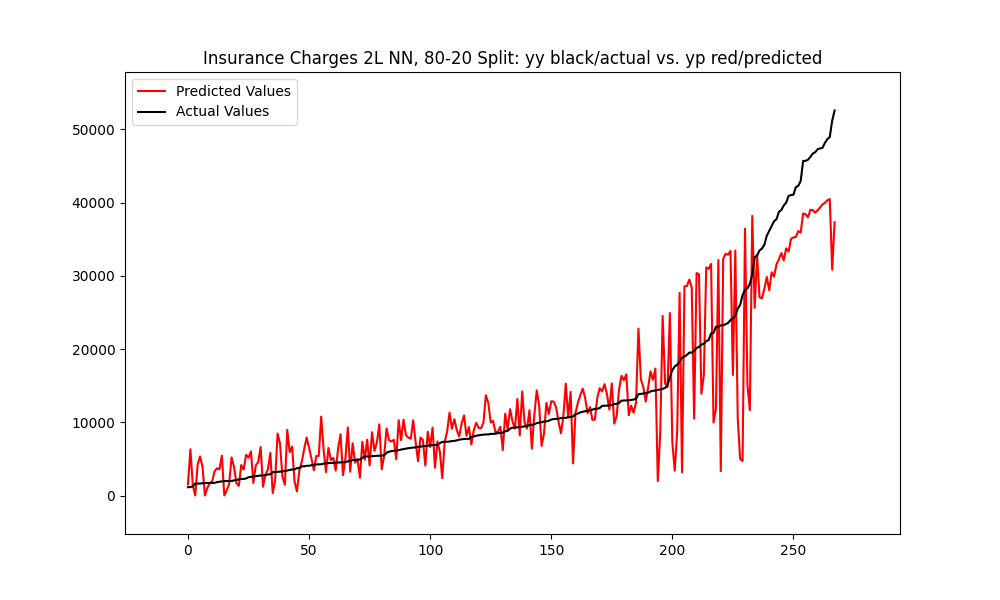
\includegraphics[width=\textwidth]{../Insurance_P2/PyTorch_2L_80_20.png}
     \end{subfigure}
     
     \caption{Insurance Charges 2 Layer Neural Network Plots\\ Top Left: Scalation In-Sample, Top Right: Scalation Out-of-Sample\\ Bottom Left: PyTorch In-Sample, Bottom Right: PyTorch Out-of-Sample\\ black: actual y-values, red: predicted y-values}
     \label{fig:Insurance Charges 2L Plots}
\end{figure}

\subsection{3 Layer Neural Network}

In Scalation, the best results were found when using lreLU as the activation function for the hidden layer, identity as the activation function for the output layer, $2\times x.dim2=16$ nodes in the hidden layer, a learning rate of $0.01$, and a batch size of $16$. The results are shown in \Cref{tab:Scalation - Insurance Charges 3L NN}. In PyTorch, the best results were found when using LeakyReLU as the activation function for the hidden layer, identity as the activation function for the output layer, $100$ nodes in the hidden layer, a learning rate of $0.01$, and a batch size of $32$. The results are shown in \Cref{tab:PyTorch - Insurance Charges 3L NN}. Plots for In-Sample and Out-of-Sample testing can be found in \Cref{fig:Insurance Charges 3L Plots}.

\begin{table}[H]
\centering
\caption{Scalation - Insurance Charges 3L NN}
\label{tab:Scalation - Insurance Charges 3L NN}
\begin{tabular}{|c|c|c|} \hline 
Metric & In-Sample & 80-20 Split \\ \hline \hline 
rSq &0.867231 & 0.817677 \\ \hline 
rSqBar &0.866432 &      0.816580 \\ \hline 
sst &5446.51 &  1128.98 \\ \hline 
sse &723.127 &  205.838 \\ \hline 
sde &0.735248 & 0.877561 \\ \hline 
mse0 &0.540454 &        0.770930 \\ \hline 
rmse &0.735156 &        0.878026 \\ \hline 
mae &0.416711 & 0.534961 \\ \hline 
smape &24.6632 &        31.2906 \\ \hline 
m &1338.00 &    267.000 \\ \hline 
dfr &8.00000 &  8.00000 \\ \hline 
df &1330.00 &   1330.00 \\ \hline 
fStat &1085.92 &        745.594 \\ \hline 
aic &-1468.87 & -326.127 \\ \hline 
bic &-1422.08 & -293.842 \\ \hline 
\end{tabular}
\end{table}

\begin{table}[H]
\centering
\caption{PyTorch - Insurance Charges 3L NN}
\label{tab:PyTorch - Insurance Charges 3L NN}
\begin{tabular}{|c|c|c|}\hline
Metric & In-Sample & 80-20 Split \\ \hline \hline
rSq & 0.8766 & 0.8891 \\ \hline
rSqBar & 0.8760 & 0.8861 \\ \hline
sst & 196074221568.3671 & 42646829902.3297 \\ \hline
sse & 24191406710.2515 & 4730156280.8836 \\ \hline
sde & 4264.8596 & 4265.3146 \\ \hline
mse0 & 18080274.0734 & 17649836.8690 \\ \hline
rmse & 4252.0906 & 4201.1709 \\ \hline
mae & 2466.8147 & 2735.5215 \\ \hline
smape & 23.6520 & 27.4890 \\ \hline
m & 1338.0000 & 268.0000 \\ \hline
dfr & 8.0000 & 8.0000 \\ \hline
df & 1330.0000 & 260.0000 \\ \hline
fStat & 1181.2260 & 260.5182 \\ \hline
aic & 22374.4243 & 4487.9115 \\ \hline
bic & 22416.0158 & 4516.6394 \\ \hline
\end{tabular}
\end{table}

\begin{figure}[H]
     \centering
     \captionsetup{justification=centering}
     % First Row
     \begin{subfigure}[b]{0.4\textwidth}
         \centering
         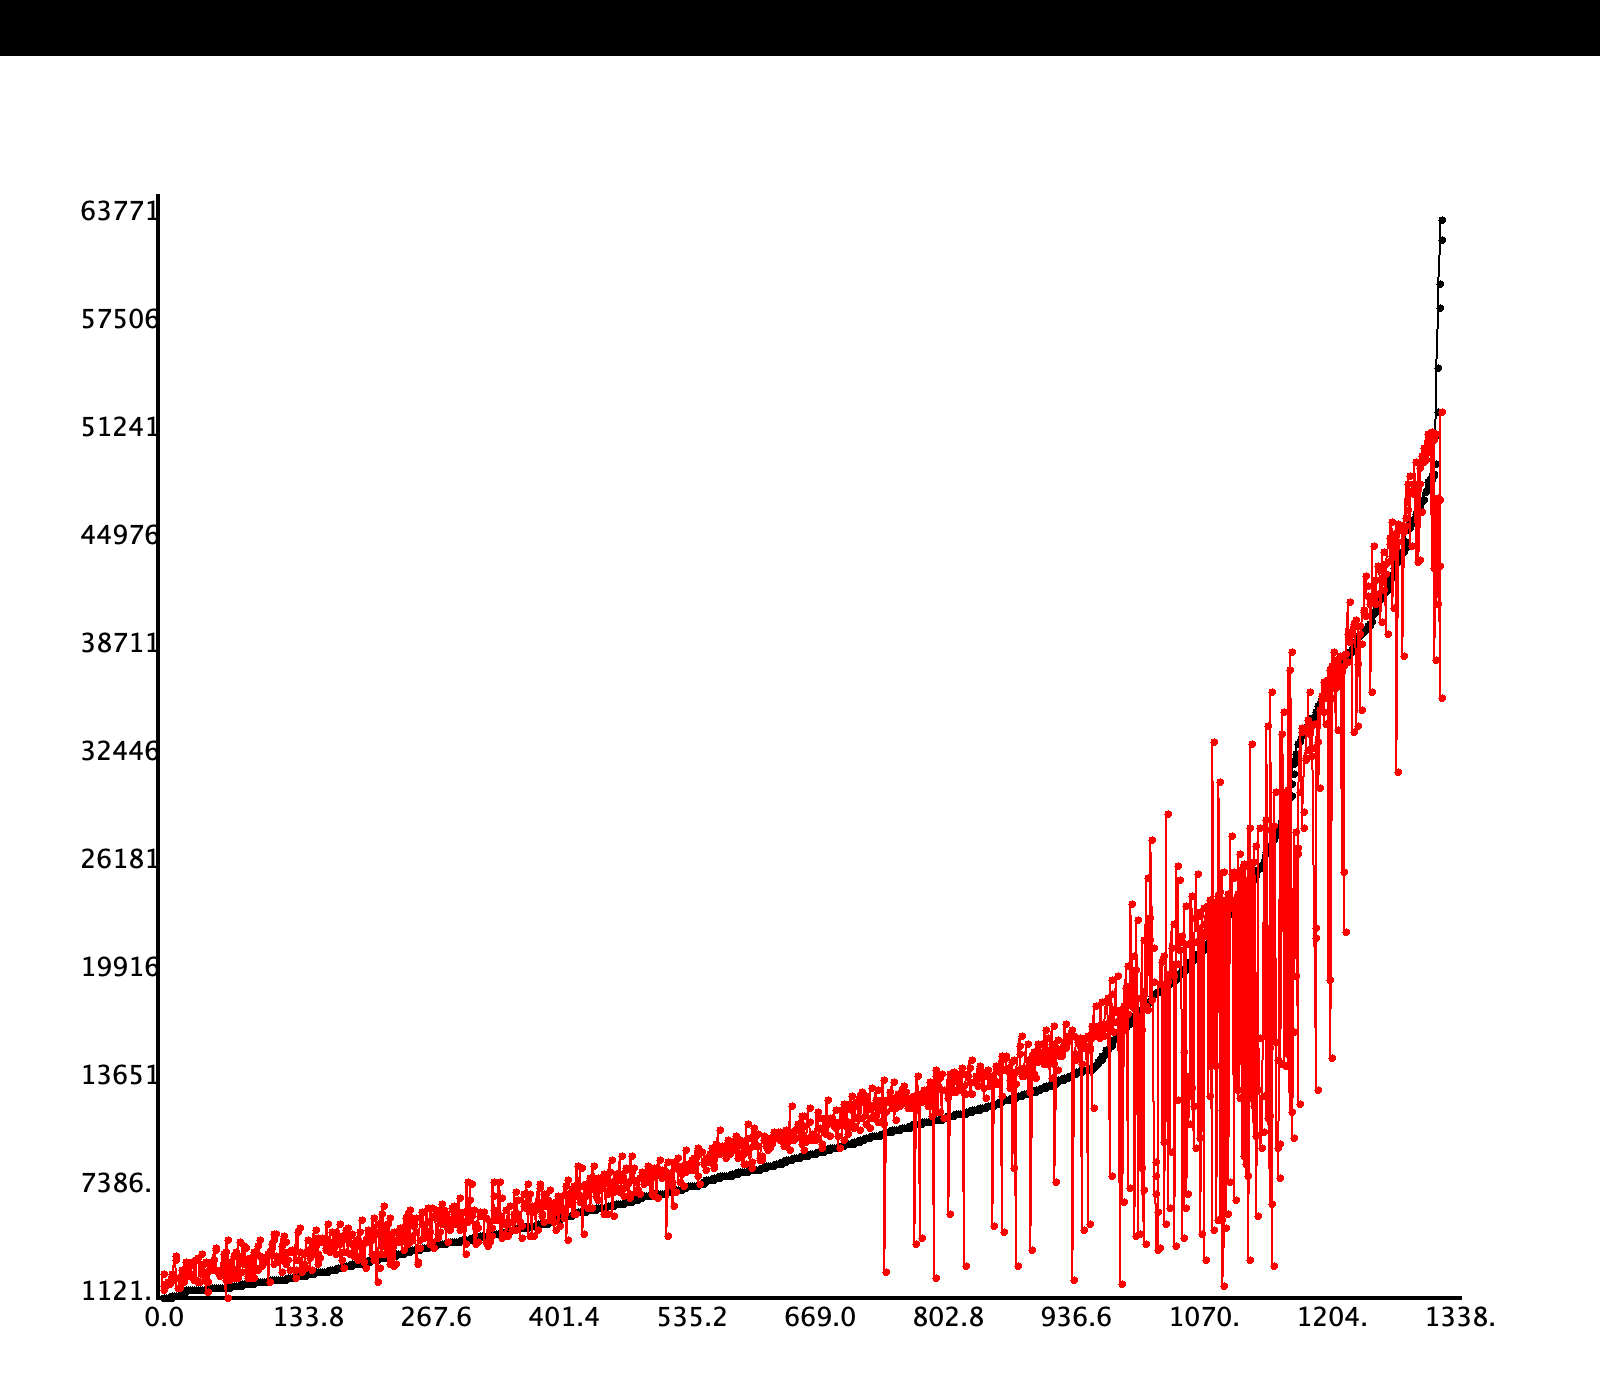
\includegraphics[width=\textwidth]{../Insurance_P2/Scalation_3L_In_Sample.png}
     \end{subfigure}
     \hfill
     \begin{subfigure}[b]{0.4\textwidth}
         \centering
         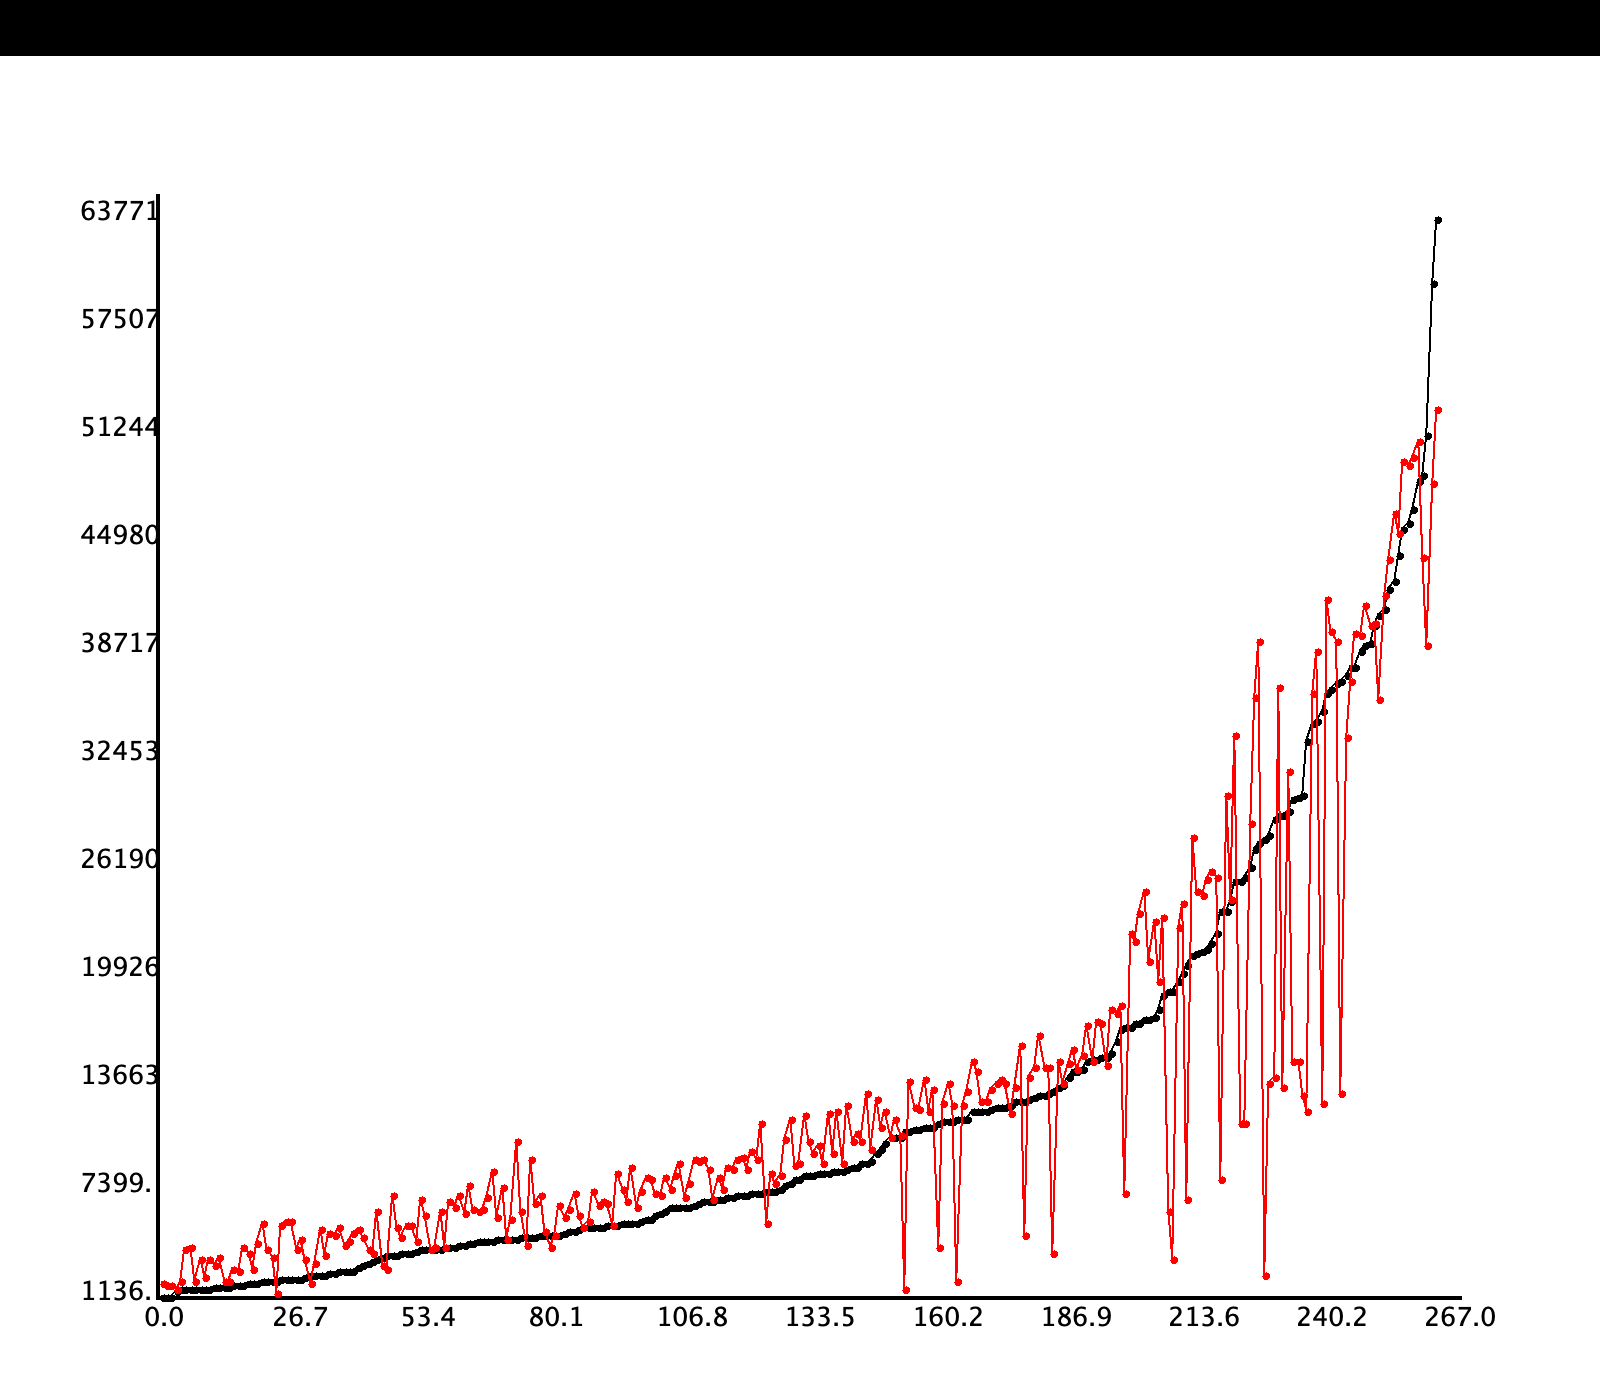
\includegraphics[width=\textwidth]{../Insurance_P2/Scalation_3L_80_20.png}
     \end{subfigure}

     \vspace{10pt} % Add some vertical spacing between rows

     % Second Row
     \begin{subfigure}[b]{0.49\textwidth}
         \centering
         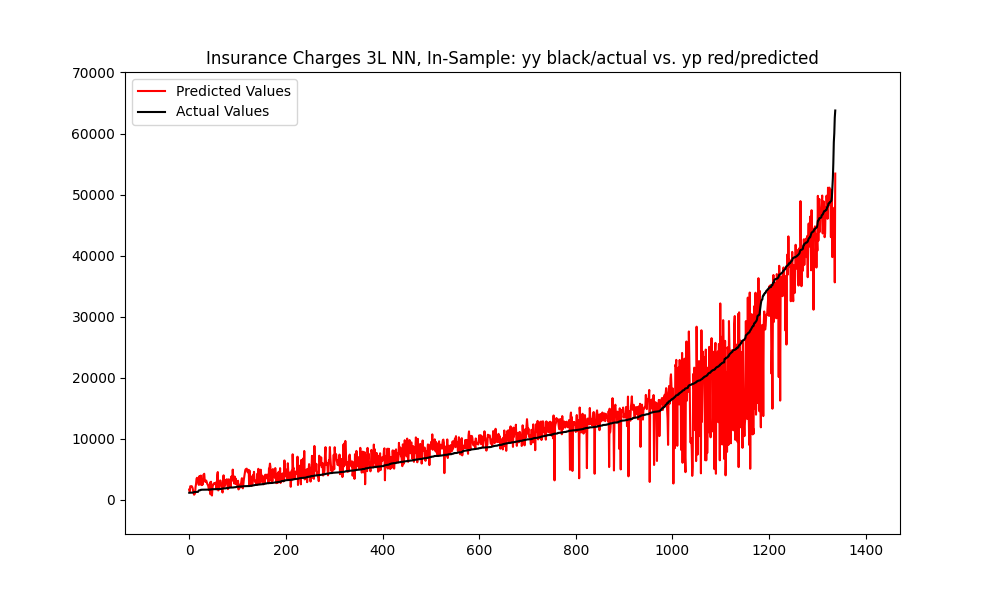
\includegraphics[width=\textwidth]{../Insurance_P2/PyTorch_3L_In_Sample.png}
     \end{subfigure}
     \hfill
     \begin{subfigure}[b]{0.49\textwidth}
         \centering
         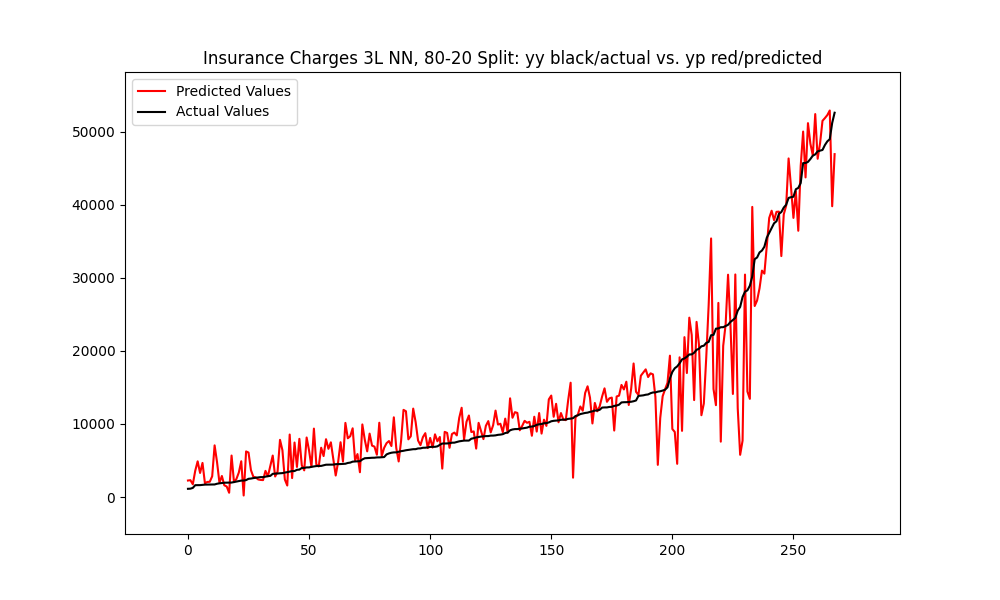
\includegraphics[width=\textwidth]{../Insurance_P2/PyTorch_3L_80_20.png}
     \end{subfigure}
     
     \caption{Insurance Charges 3 Layer Neural Network Plots\\ Top Left: Scalation In-Sample, Top Right: Scalation Out-of-Sample\\ Bottom Left: PyTorch In-Sample, Bottom Right: PyTorch Out-of-Sample\\ black: actual y-values, red: predicted y-values}
     \label{fig:Insurance Charges 3L Plots}
\end{figure}

\subsection{4 Layer Neural Network}

\section{Summary}

\subsection{Auto MPG}

\begin{table}[H]
\centering
\caption{Scalation: - Auto MPG In-Sample QoF Comparison}
\label{tab:Scalation: - Auto MPG In-Sample QoF Comparison}
\begin{tabular}{|c|c|c|} \hline 
Metric & 2 Layer NN & 3 Layer NN \\ \hline \hline 
rSq & 0.727231 & 0.930275 \\ \hline 
rSqBar & 0.722259 & 0.928822 \\ \hline 
sst & 23819.0 & 23819.0 \\ \hline 
sse & 6497.08 & 1660.78 \\ \hline 
sde & 3.39572 & 2.05245 \\ \hline 
mse0 & 16.5742 & 4.23669 \\ \hline 
rmse & 4.07114 & 2.05832 \\ \hline 
mae & 3.31165 & 1.50903 \\ \hline 
smape & 14.4265 & 6.54887 \\ \hline 
m & 392.000 & 392.000 \\ \hline 
dfr & 7.00000 & 8.00000 \\ \hline 
df & 384.000 & 384.000 \\ \hline 
fStat & 146.255 & 640.418 \\ \hline 
aic & -1105.39 & -821.212 \\ \hline 
bic & -1073.62 & -785.471 \\ \hline 
\end{tabular}
\end{table}

\begin{table}[H]
\centering
\caption{PyTorch: - Auto MPG In-Sample QoF Comparison}
\label{tab:PyTorch: - Auto MPG In-Sample QoF Comparison}
\begin{tabular}{|c|c|c|} \hline 
Metric & 2 Layer NN & 3 Layer NN \\ \hline \hline 
rSq & 0.8232 & 0.8855 \\ \hline 
rSqBar & 0.8199 & 0.8835 \\ \hline 
sst & 23818.9935 & 23818.9935 \\ \hline 
sse & 4211.9875 & 2726.1212 \\ \hline 
sde & 3.3119 & 2.6644 \\ \hline 
mse0 & 10.7449 & 6.9544 \\ \hline 
rmse & 3.2779 & 2.6371 \\ \hline 
mae & 2.4941 & 1.8997 \\ \hline 
smape & 11.4175 & 8.0857 \\ \hline 
m & 392.0000 & 392.0000 \\ \hline 
dfr & 8.0000 & 8.0000 \\ \hline 
df & 384.0000 & 384.0000 \\ \hline 
fStat & 223.4423 & 371.3914 \\ \hline 
aic & 946.7758 & 776.2343 \\ \hline 
bic & 978.5459 & 808.0044 \\ \hline 
\end{tabular}
\end{table}

\begin{table}[H]
\centering
\caption{Scalation: - Auto MPG Out-of-Sample QoF Comparison}
\label{tab:Scalation: - Auto MPG Out-of-Sample QoF Comparison}
\begin{tabular}{|c|c|c|} \hline 
Metric & 2 Layer NN & 3 Layer NN \\ \hline \hline 
rSq & 0.836932 & 0.868516 \\ \hline 
rSqBar & 0.833959 & 0.865777 \\ \hline 
sst & 4731.23 & 4731.23 \\ \hline 
sse & 771.514 & 622.081 \\ \hline 
sde & 3.16498 & 2.79802 \\ \hline 
mse0 & 9.89121 & 7.97540 \\ \hline 
rmse & 3.14503 & 2.82407 \\ \hline 
mae & 2.36625 & 2.03520 \\ \hline 
smape & 10.7664 & 8.62759 \\ \hline 
m & 78.0000 & 78.0000 \\ \hline 
dfr & 7.00000 & 8.00000 \\ \hline 
df & 384.000 & 384.000 \\ \hline 
fStat & 281.549 & 317.064 \\ \hline 
aic & -184.051 & -173.675 \\ \hline 
bic & -165.198 & -152.464 \\ \hline 
\end{tabular}
\end{table}

\begin{table}[H]
\centering
\caption{PyTorch: - Auto MPG Out-of-Sample QoF Comparison}
\label{tab:PyTorch: - Auto MPG Out-of-Sample QoF Comparison}
\begin{tabular}{|c|c|c|} \hline 
Metric & 2 Layer NN & 3 Layer NN \\ \hline \hline 
rSq & 0.8391 & 0.9095 \\ \hline 
rSqBar & 0.8232 & 0.9005 \\ \hline 
sst & 4910.2699 & 4910.2699 \\ \hline 
sse & 790.2830 & 444.5322 \\ \hline 
sde & 3.3363 & 2.5022 \\ \hline 
mse0 & 10.0036 & 5.6270 \\ \hline 
rmse & 3.1628 & 2.3721 \\ \hline 
mae & 2.4081 & 1.6043 \\ \hline 
smape & 11.1501 & 7.0419 \\ \hline 
m & 79.0000 & 79.0000 \\ \hline 
dfr & 8.0000 & 8.0000 \\ \hline 
df & 71.0000 & 71.0000 \\ \hline 
fStat & 46.2681 & 89.1576 \\ \hline 
aic & 197.9325 & 152.4784 \\ \hline 
bic & 216.8881 & 171.4340 \\ \hline 
\end{tabular}
\end{table}

\subsection{California House Prices}

\begin{table}[H]
\centering
\caption{Scalation: - California House Prices In-Sample QoF Comparison}
\label{tab:Scalation: - California House Prices In-Sample QoF Comparison}
\begin{tabular}{|c|c|c|} \hline 
Metric & 2 Layer NN & 3 Layer NN \\ \hline \hline 
rSq & 0.633776 & 0.779769 \\ \hline 
rSqBar & 0.633579 & 0.779639 \\ \hline 
sst & 2.72264e+14 & 27226.4 \\ \hline 
sse & 9.97097e+13 & 5996.11 \\ \hline 
sde & 69653.2 & 0.541323 \\ \hline 
mse0 & 4.87984e+09 & 0.293452 \\ \hline 
rmse & 69855.8 & 0.541712 \\ \hline 
mae & 51821.3 & 0.371532 \\ \hline 
smape & 26.8854 & 19.3019 \\ \hline 
m & 20433.0 & 20433.0 \\ \hline 
dfr & 11.0000 & 12.0000 \\ \hline 
df & 20421.0 & 20421.0 \\ \hline 
fStat & 3212.73 & 6025.36 \\ \hline 
aic & -256883 & -16441.3 \\ \hline 
bic & -256788 & -16338.3 \\ \hline 
\end{tabular}
\end{table}

\begin{table}[H]
\centering
\caption{PyTorch: - California House Prices In-Sample QoF Comparison}
\label{tab:PyTorch: - California House Prices In-Sample QoF Comparison}
\begin{tabular}{|c|c|c|} \hline 
Metric & 2 Layer NN & 3 Layer NN \\ \hline \hline 
rSq & 0.6468 & 0.8057 \\ \hline 
rSqBar & 0.6466 & 0.8056 \\ \hline 
sst & 272264434648930.1875 & 272264434648930.1250 \\ \hline 
sse & 96172625731084.4375 & 52901444882088.6094 \\ \hline 
sde & 68625.7706 & 50897.3609 \\ \hline 
mse0 & 4706730569.7198 & 2589019961.9287 \\ \hline 
rmse & 68605.6162 & 50882.4131 \\ \hline 
mae & 49654.9430 & 34838.6035 \\ \hline 
smape & 26.7647 & 18.1115 \\ \hline 
m & 20433.0000 & 20433.0000 \\ \hline 
dfr & 12.0000 & 12.0000 \\ \hline 
df & 20421.0000 & 20421.0000 \\ \hline 
fStat & 3115.8995 & 7056.5363 \\ \hline 
aic & 455113.0754 & 442899.9831 \\ \hline 
bic & 455208.1743 & 442995.0819 \\ \hline 
\end{tabular}
\end{table}

\begin{table}[H]
\centering
\caption{Scalation: - California House Prices Out-of-Sample QoF Comparison}
\label{tab:Scalation: - California House Prices Out-of-Sample QoF Comparison}
\begin{tabular}{|c|c|c|} \hline 
Metric & 2 Layer NN & 3 Layer NN \\ \hline \hline 
rSq & 0.630655 & 0.756155 \\ \hline 
rSqBar & 0.630456 & 0.756012 \\ \hline 
sst & 5.31945e+13 & 5319.45 \\ \hline 
sse & 1.96471e+13 & 1297.12 \\ \hline 
sde & 69346.2 & 0.562612 \\ \hline 
mse0 & 4.80840e+09 & 0.317454 \\ \hline 
rmse & 69342.6 & 0.563431 \\ \hline 
mae & 50737.2 & 0.389204 \\ \hline 
smape & 26.5678 & 20.5293 \\ \hline 
m & 4086.00 & 4086.00 \\ \hline 
dfr & 11.0000 & 12.0000 \\ \hline 
df & 20421.0 & 20421.0 \\ \hline 
fStat & 3169.89 & 5277.08 \\ \hline 
aic & -51319.7 & -3427.61 \\ \hline 
bic & -51243.9 & -3345.51 \\ \hline 
\end{tabular}
\end{table}

\begin{table}[H]
\centering
\caption{PyTorch: - California House Prices Out-of-Sample QoF Comparison}
\label{tab:PyTorch: - California House Prices Out-of-Sample QoF Comparison}
\begin{tabular}{|c|c|c|} \hline 
Metric & 2 Layer NN & 3 Layer NN \\ \hline \hline 
rSq & 0.6516 & 0.7961 \\ \hline 
rSqBar & 0.6506 & 0.7956 \\ \hline 
sst & 54723646809444.8438 & 54723646809444.8281 \\ \hline 
sse & 19066274074331.2266 & 11156430483920.8633 \\ \hline 
sde & 68402.0487 & 52323.7456 \\ \hline 
mse0 & 4665102538.3732 & 2729735865.8970 \\ \hline 
rmse & 68301.5559 & 52246.8742 \\ \hline 
mae & 50131.4253 & 35574.6590 \\ \hline 
smape & 26.6343 & 18.1492 \\ \hline 
m & 4087.0000 & 4087.0000 \\ \hline 
dfr & 12.0000 & 12.0000 \\ \hline 
df & 4075.0000 & 4075.0000 \\ \hline 
fStat & 635.0821 & 1326.1142 \\ \hline 
aic & 91014.4163 & 88824.1727 \\ \hline 
bic & 91090.2031 & 88899.9595 \\ \hline 
\end{tabular}
\end{table}

\subsection{Insurance Charges}

\begin{table}[H]
\centering
\caption{Scalation: - Insurance Charges In-Sample QoF Comparison}
\label{tab:Scalation: - Insurance Charges In-Sample QoF Comparison}
\begin{tabular}{|c|c|c|} \hline 
Metric & 2 Layer NN & 3 Layer NN \\ \hline \hline 
rSq & 0.722979 & 0.867231 \\ \hline 
rSqBar & 0.721521 & 0.866432 \\ \hline 
sst & 1.96074e+11 & 5446.51 \\ \hline 
sse & 5.43167e+10 & 723.127 \\ \hline 
sde & 6346.14 & 0.735248 \\ \hline 
mse0 & 4.05954e+07 & 0.540454 \\ \hline 
rmse & 6371.45 & 0.735156 \\ \hline 
mae & 4519.55 & 0.416711 \\ \hline 
smape & 39.5992 & 24.6632 \\ \hline 
m & 1338.00 & 1338.00 \\ \hline 
dfr & 7.00000 & 8.00000 \\ \hline 
df & 1330.00 & 1330.00 \\ \hline 
fStat & 495.869 & 1085.92 \\ \hline 
aic & -13602.9 & -1468.87 \\ \hline 
bic & -13561.3 & -1422.08 \\ \hline 
\end{tabular}
\end{table}

\begin{table}[H]
\centering
\caption{PyTorch: - Insurance Charges In-Sample QoF Comparison}
\label{tab:PyTorch: - Insurance Charges In-Sample QoF Comparison}
\begin{tabular}{|c|c|c|} \hline 
Metric & 2 Layer NN & 3 Layer NN \\ \hline \hline 
rSq & 0.7516 & 0.8766 \\ \hline 
rSqBar & 0.7503 & 0.8760 \\ \hline 
sst & 196074221568.3671 & 196074221568.3671 \\ \hline 
sse & 48702200251.0962 & 24191406710.2515 \\ \hline 
sde & 6051.2970 & 4264.8596 \\ \hline 
mse0 & 36399252.8035 & 18080274.0734 \\ \hline 
rmse & 6033.1793 & 4252.0906 \\ \hline 
mae & 4158.4738 & 2466.8147 \\ \hline 
smape & 39.1264 & 23.6520 \\ \hline 
m & 1338.0000 & 1338.0000 \\ \hline 
dfr & 8.0000 & 8.0000 \\ \hline 
df & 1330.0000 & 1330.0000 \\ \hline 
fStat & 503.0696 & 1181.2260 \\ \hline 
aic & 23310.6587 & 22374.4243 \\ \hline 
bic & 23352.2501 & 22416.0158 \\ \hline 
\end{tabular}
\end{table}

\begin{table}[H]
\centering
\caption{Scalation: - Insurance Charges Out-of-Sample QoF Comparison}
\label{tab:Scalation: - Insurance Charges Out-of-Sample QoF Comparison}
\begin{tabular}{|c|c|c|} \hline 
Metric & 2 Layer NN & 3 Layer NN \\ \hline \hline 
rSq & 0.682065 & 0.817677 \\ \hline 
rSqBar & 0.680392 & 0.816580 \\ \hline 
sst & 4.06432e+10 & 1128.98 \\ \hline 
sse & 1.29219e+10 & 205.838 \\ \hline 
sde & 6966.63 & 0.877561 \\ \hline 
mse0 & 4.83965e+07 & 0.770930 \\ \hline 
rmse & 6956.76 & 0.878026 \\ \hline 
mae & 4729.99 & 0.534961 \\ \hline 
smape & 41.9288 & 31.2906 \\ \hline 
m & 267.000 & 267.000 \\ \hline 
dfr & 7.00000 & 8.00000 \\ \hline 
df & 1330.00 & 1330.00 \\ \hline 
fStat & 407.607 & 745.594 \\ \hline 
aic & -2725.13 & -326.127 \\ \hline 
bic & -2696.43 & -293.842 \\ \hline 
\end{tabular}
\end{table}

\begin{table}[H]
\centering
\caption{PyTorch: - Insurance Charges Out-of-Sample QoF Comparison}
\label{tab:PyTorch: - Insurance Charges Out-of-Sample QoF Comparison}
\begin{tabular}{|c|c|c|} \hline 
Metric & 2 Layer NN & 3 Layer NN \\ \hline \hline 
rSq & 0.8007 & 0.8891 \\ \hline 
rSqBar & 0.7953 & 0.8861 \\ \hline 
sst & 42646829902.3297 & 42646829902.3297 \\ \hline 
sse & 8498989265.5920 & 4730156280.8836 \\ \hline 
sde & 5717.3788 & 4265.3146 \\ \hline 
mse0 & 31712646.5134 & 17649836.8690 \\ \hline 
rmse & 5631.3983 & 4201.1709 \\ \hline 
mae & 3932.9280 & 2735.5215 \\ \hline 
smape & 36.6337 & 27.4890 \\ \hline 
m & 268.0000 & 268.0000 \\ \hline 
dfr & 8.0000 & 8.0000 \\ \hline 
df & 260.0000 & 260.0000 \\ \hline 
fStat & 130.5808 & 260.5182 \\ \hline 
aic & 4644.9566 & 4487.9115 \\ \hline 
bic & 4673.6845 & 4516.6394 \\ \hline 
\end{tabular}
\end{table}

\end{document}